% Supplementary Information, preserving the v1p1 scientific content.
\documentclass[11pt,a4paper]{article}
\usepackage[margin=20mm]{geometry}
\usepackage{amsmath,amssymb,graphicx,xcolor,tikz}
\usepackage[numbers,sort&compress]{natbib}
\usepackage{xr-hyper}
\usepackage[hidelinks]{hyperref}
\externaldocument[main-]{build/manuscript}[manuscript.pdf]
\renewcommand{\theequation}{S\arabic{equation}}
\renewcommand{\thefigure}{S\arabic{figure}}
\renewcommand{\thetable}{S\arabic{table}}
\setcounter{secnumdepth}{0}
\allowdisplaybreaks
\setlength{\emergencystretch}{1em}
\begin{document}
\begin{center}
{\Large\bfseries Supplementary Information}\par\medskip
{\large Blast freezing a black hole}\par\medskip
Shoaib Akhtar and Xiao-Liang Qi
\end{center}
\bigskip
\section*{S1. Microscopic model and evaporation protocol}
The main text and Methods describe the quench schematically as initially
decoupled \(\eta\) and \(\chi\) SYK sectors that merge at \(t_{\rm ev}\). Here
we give the microscopic realization of that shorthand model, including the
relative normalization of the pure and mixed interactions and a slightly more
general formation-and-evaporation protocol. Using the parameter \(s\) defined
in Methods, the one-sided Hamiltonian is
\begin{equation}
\begin{aligned}
H[\eta,\chi;J]
&=
i^{p/2}s^{-p/2}l_\eta(t)
\sum_{I_p}J_{I_p}\eta_{I_p}
+
i^{p/2}(1-s)^{-p/2}l_\chi(t)
\sum_{K_p}J_{K_p}\chi_{K_p}
\\
&\quad
+i^{p/2}l_c(t)
\sum_{m=1}^{p-1}
\sum_{I_m,K_{p-m}}
J_{I_m;K_{p-m}}\eta_{I_m}\chi_{K_{p-m}} .
\end{aligned}
\label{eq:S-one-sided-H}
\end{equation}
Here \(p/2\) is even, matching the reflected-copy convention used below. The multi-index
\(I_m=(i_1,\ldots,i_m)\) is an increasing \(m\)-tuple of
\(\eta\)-indices, and
\(\eta_{I_m}\equiv\eta_{i_1}\cdots\eta_{i_m}\).
Similarly, \(K_n=(k_1,\ldots,k_n)\) is an increasing \(n\)-tuple of
\(\chi\)-indices, with
\(\chi_{K_n}\equiv\chi_{k_1}\cdots\chi_{k_n}\).

All couplings associated with distinct index sets are independent Gaussian
random variables with zero mean and common variance
\begin{equation}
\begin{aligned}
\overline{J_{I_p}^{\,2}}
=
\overline{J_{K_p}^{\,2}}
=
\overline{J_{I_m;K_{p-m}}^{\,2}}
&=
J^2\frac{(p-1)!}{(N_\eta+N_\chi)^{p-1}}
\\
&=
\mathcal J^2\frac{2^{p-1}}{p}
\frac{(p-1)!}{(N_\eta+N_\chi)^{p-1}},
\qquad 1\leq m\leq p-1 .
\end{aligned}
\label{eq:S-disorder}
\end{equation}
The left and right copies use the same disorder realization.

A sharp evaporation protocol that realizes the shorthand Hamiltonian in
Methods is
\begin{equation}
\begin{aligned}
l_\eta(t)
&=
a\,s^{1/2}\theta(t_{\rm ev}-t)
+s^{p/2}\theta(t-t_{\rm ev}),
\\
l_\chi(t)
&=
b\,(1-s)^{1/2}\theta(t_{\rm ev}-t)
+(1-s)^{p/2}\theta(t-t_{\rm ev}),
\\
l_c(t)
&=
\theta(t-t_{\rm ev}) .
\end{aligned}
\label{eq:S-l-protocol}
\end{equation}
For \(t<t_{\rm ev}\), \(l_c=0\), while the total coefficients of the pure
\(\eta\) and \(\chi\) interactions are
\(a\,s^{(1-p)/2}\) and \(b\,(1-s)^{(1-p)/2}\), respectively. Together with
Eq.~\eqref{eq:S-disorder}, these give the standard SYK normalization for
systems of sizes \(N_\eta\) and \(N_\chi\), with interaction scales controlled
by \(a\) and \(b\); the main calculation uses \(a=b=1\). For
\(t>t_{\rm ev}\),
\(s^{-p/2}l_\eta=(1-s)^{-p/2}l_\chi=l_c=1\), so the pure and mixed
\(p\)-body monomials have the same variance and assemble into
\(H_{\rm SYK}[\eta\oplus\chi]\).

The left-right bilinear couplings in the doubled Hamiltonian can be
parameterized more generally as
\begin{equation}
\begin{aligned}
\mu_\eta(t)
&=
\mu\left[
c\,\theta(-t)+\nu\,\theta(t-t_{\rm ev})
\right],
\\
\mu_\chi(t)
&=
\mu\left[
d\,\theta(t_{\rm ev}-t)+\theta(t-t_{\rm ev})
\right].
\end{aligned}
\label{eq:S-bilinear-protocol}
\end{equation}
Here \(c,d,\nu\) are dimensionless constants. The evaporation protocol used
in the main calculation is \(c=\nu=0\), \(d=1\), and \(\mu=\mu_0\), for which
\(\mu_\eta(t)=0\) and \(\mu_\chi(t)=\mu_0\). The
formation-and-evaporation extension discussed in the main text and Methods instead takes
\(c\neq0\), \(\nu=0\), and \(d=1\): the \(\eta\) bilinear is present for
\(t<0\), is switched off at \(t=0\), and the \(\eta\)-\(\chi\) interaction is
subsequently switched on at \(t_{\rm ev}\). The more general choices
\(d\neq1\) and \(\nu\neq0\) would allow, respectively, a change of the bath
bilinear at \(t_{\rm ev}\) and an \(\eta\) bilinear after evaporation.

More generally, the changes in \(l_\eta,l_\chi,l_c,\mu_\eta\), and
\(\mu_\chi\) may occur at distinct times, and the step functions may be
replaced by smooth profiles, including the gradual evaporation mentioned in
the main text and Methods. The calculations presented here use the sharp
profiles above.

\section*{S2. Bilocal effective theory}

\noindent
Methods summarizes the large-\(N\) and large-\(p\) equations used in the main
text. Here we derive those equations from the disorder-averaged bilocal action
and spell out the contour conventions.

\paragraph*{Large-\(N\) scaling and real-time contour.}

We first take \(N_\eta,N_\chi\to\infty\) at fixed \(s\) and fixed \(p\).
With the normalization introduced in Sec.~S1, the decoupled \(\eta\) and
\(\chi\) sectors contribute at order \(N_\eta\) and \(N_\chi\), respectively,
whereas the post-evaporation action is of order \(N_\eta+N_\chi\). Throughout
this section, \(a,b\in\{R,L\}\) denote copy indices and should not be confused
with the protocol constants \(a\) and \(b\) in Sec.~S1.

The calculation is performed on the Schwinger--Keldysh contour shown in
Fig.~\ref{fig:S-kb-contour}, defined by
\begin{equation}
\mathcal C
=
\mathcal C^+_{\beta/4}
\cup
\mathcal C^+
\cup
\mathcal C^-
\cup
\mathcal C^-_{\beta/4}.
\label{eq:S-kb-contour}
\end{equation}
The forward and backward real-time branches \(\mathcal C^+\) and
\(\mathcal C^-\) compute in-in observables, while the vertical segments
prepare the common-inverse-temperature \(\beta\) thermofield-double data
used in the finite-\(p\) calculation of Sec.~S5. The analytic solutions in
Sec.~S3 instead allow independent initial data for the two decoupled sectors:
a thermal \(\eta\) state and a stationary coupled \(\chi\) bath. The
real-time equations below apply to both preparations, with the corresponding
Euclidean boundary data.

\begin{figure}
    \centering

\tikzset{every picture/.style={line width=0.75pt}}

\begin{tikzpicture}[x=0.75pt,y=0.75pt,yscale=-1,xscale=1]

\draw    (100,220) -- (518,220) ;
\draw [shift={(520,220)}, rotate = 180] [color={rgb, 255:red, 0; green, 0; blue, 0 }  ][line width=0.75]    (10.93,-3.29) .. controls (6.95,-1.4) and (3.31,-0.3) .. (0,0) .. controls (3.31,0.3) and (6.95,1.4) .. (10.93,3.29)   ;

\draw    (160,360) -- (160,82) ;
\draw [shift={(160,80)}, rotate = 90] [color={rgb, 255:red, 0; green, 0; blue, 0 }  ][line width=0.75]    (10.93,-3.29) .. controls (6.95,-1.4) and (3.31,-0.3) .. (0,0) .. controls (3.31,0.3) and (6.95,1.4) .. (10.93,3.29)   ;

\draw [color={rgb, 255:red, 208; green, 2; blue, 27 }  ,draw opacity=1 ]   (160,190) -- (480,190) ;
\draw [shift={(325,190)}, rotate = 180] [fill={rgb, 255:red, 208; green, 2; blue, 27 }  ,fill opacity=1 ][line width=0.08]  [draw opacity=0] (10.72,-5.15) -- (0,0) -- (10.72,5.15) -- (7.12,0) -- cycle    ;

\draw [color={rgb, 255:red, 208; green, 2; blue, 27 }  ,draw opacity=1 ] [dash pattern={on 0.84pt off 2.51pt}]  (480,190) -- (510,190) ;

\draw [color={rgb, 255:red, 208; green, 2; blue, 27 }  ,draw opacity=1 ]   (160,250) -- (480,250) ;
\draw [shift={(313.5,250)}, rotate = 0] [fill={rgb, 255:red, 208; green, 2; blue, 27 }  ,fill opacity=1 ][line width=0.08]  [draw opacity=0] (10.72,-5.15) -- (0,0) -- (10.72,5.15) -- (7.12,0) -- cycle    ;

\draw [color={rgb, 255:red, 208; green, 2; blue, 27 }  ,draw opacity=1 ] [dash pattern={on 0.84pt off 2.51pt}]  (480,250) -- (510,250) ;

\draw [color={rgb, 255:red, 208; green, 2; blue, 27 }  ,draw opacity=1 ]   (160,330) -- (160,250) ;
\draw [shift={(160,296.5)}, rotate = 270] [fill={rgb, 255:red, 208; green, 2; blue, 27 }  ,fill opacity=1 ][line width=0.08]  [draw opacity=0] (10.72,-5.15) -- (0,0) -- (10.72,5.15) -- (7.12,0) -- cycle    ;

\draw  [color={rgb, 255:red, 65; green, 117; blue, 5 }  ,draw opacity=1 ][fill={rgb, 255:red, 65; green, 117; blue, 5 }  ,fill opacity=1 ] (156.21,250) .. controls (156.21,247.91) and (157.91,246.21) .. (160,246.21) .. controls (162.09,246.21) and (163.79,247.91) .. (163.79,250) .. controls (163.79,252.09) and (162.09,253.79) .. (160,253.79) .. controls (157.91,253.79) and (156.21,252.09) .. (156.21,250) -- cycle ;

\draw  [color={rgb, 255:red, 65; green, 117; blue, 5 }  ,draw opacity=1 ][fill={rgb, 255:red, 65; green, 117; blue, 5 }  ,fill opacity=1 ] (156.21,330) .. controls (156.21,327.91) and (157.91,326.21) .. (160,326.21) .. controls (162.09,326.21) and (163.79,327.91) .. (163.79,330) .. controls (163.79,332.09) and (162.09,333.79) .. (160,333.79) .. controls (157.91,333.79) and (156.21,332.09) .. (156.21,330) -- cycle ;

\draw [color={rgb, 255:red, 208; green, 2; blue, 27 }  ,draw opacity=1 ]   (160,190) -- (160,110) ;
\draw [shift={(160,156.5)}, rotate = 270] [fill={rgb, 255:red, 208; green, 2; blue, 27 }  ,fill opacity=1 ][line width=0.08]  [draw opacity=0] (10.72,-5.15) -- (0,0) -- (10.72,5.15) -- (7.12,0) -- cycle    ;

\draw  [color={rgb, 255:red, 65; green, 117; blue, 5 }  ,draw opacity=1 ][fill={rgb, 255:red, 65; green, 117; blue, 5 }  ,fill opacity=1 ] (156.21,110) .. controls (156.21,107.91) and (157.91,106.21) .. (160,106.21) .. controls (162.09,106.21) and (163.79,107.91) .. (163.79,110) .. controls (163.79,112.09) and (162.09,113.79) .. (160,113.79) .. controls (157.91,113.79) and (156.21,112.09) .. (156.21,110) -- cycle ;

\draw  [color={rgb, 255:red, 65; green, 117; blue, 5 }  ,draw opacity=1 ][fill={rgb, 255:red, 65; green, 117; blue, 5 }  ,fill opacity=1 ] (156.21,190) .. controls (156.21,187.91) and (157.91,186.21) .. (160,186.21) .. controls (162.09,186.21) and (163.79,187.91) .. (163.79,190) .. controls (163.79,192.09) and (162.09,193.79) .. (160,193.79) .. controls (157.91,193.79) and (156.21,192.09) .. (156.21,190) -- cycle ;

\draw (103,181) node [anchor=north west][inner sep=0.75pt]   [align=left] {$\displaystyle t_{0} +i\epsilon $};

\draw (104,241) node [anchor=north west][inner sep=0.75pt]   [align=left] {$\displaystyle t_{0} -i\epsilon $};

\draw (521,211) node [anchor=north west][inner sep=0.75pt]   [align=left] {$\displaystyle \text{Re}( t)$};

\draw (141,62) node [anchor=north west][inner sep=0.75pt]   [align=left] {$\displaystyle \text{Im}( t)$};

\draw (104,321) node [anchor=north west][inner sep=0.75pt]   [align=left] {$\displaystyle t_{0} -i\frac{\beta }{4}$};

\draw (101,92) node [anchor=north west][inner sep=0.75pt]   [align=left] {$\displaystyle t_{0} +i\frac{\beta }{4}$};

\draw (311,159) node [anchor=north west][inner sep=0.75pt]   [align=left] {$\displaystyle \mathcal{C}^{+}$};

\draw (311,262) node [anchor=north west][inner sep=0.75pt]   [align=left] {$\displaystyle \mathcal{C}^{-}$};

\draw (171,139) node [anchor=north west][inner sep=0.75pt]   [align=left] {$\displaystyle \mathcal{C}_{\beta /4}^{+}$};

\draw (171,278) node [anchor=north west][inner sep=0.75pt]   [align=left] {$\displaystyle \mathcal{C}_{\beta /4}^{-}$};

\end{tikzpicture}
\caption{\textbf{Contour for real-time evolution and TFD preparation.}
The horizontal branches \(\mathcal C^+\) and \(\mathcal C^-\) describe
forward and backward real-time evolution, while
\(\mathcal C^+_{\beta/4}\) and \(\mathcal C^-_{\beta/4}\) prepare the initial
thermofield-double data. The endpoint conditions are given in
Eq.~\eqref{eq:S-tfd-gluing}.}
\label{fig:S-kb-contour}
\end{figure}

For each species \(\psi=\eta,\chi\), define
\begin{equation}
c^\psi_j
=
\frac{\psi^L_j+i\psi^R_j}{\sqrt{2}},
\qquad
\left(c^\psi_j\right)^\dagger
=
\frac{\psi^L_j-i\psi^R_j}{\sqrt{2}} .
\label{eq:S-c-def}
\end{equation}
The reference state \(\lvert\mathbf 1\rangle\) is annihilated by all
\(c^\psi_j\). Equivalently,
\begin{equation}
\psi^L_j\lvert\mathbf 1\rangle
=
-i\psi^R_j\lvert\mathbf 1\rangle,
\qquad
\langle\mathbf 1\rvert\psi^L_j
=
i\langle\mathbf 1\rvert\psi^R_j .
\label{eq:S-identity-gluing}
\end{equation}
The thermofield-double state is prepared by Euclidean evolution,
\begin{equation}
\lvert\mathrm{TFD}\rangle
=
\frac{1}{\sqrt{Z_\beta}}
e^{-\frac{\beta}{4}(H^R+H^L)}
\lvert\mathbf 1\rangle .
\label{eq:S-tfd-state}
\end{equation}
This representation fixes the endpoint conditions
\begin{equation}
\begin{aligned}
\psi^L_j(t_0+i\beta/4)
&=
-i\psi^R_j(t_0+i\beta/4),
\\
\psi^L_j(t_0-i\beta/4)
&=
i\psi^R_j(t_0-i\beta/4).
\end{aligned}
\label{eq:S-tfd-gluing}
\end{equation}

Define the contour-ordered two-point function by
\begin{equation}
G^\psi_{ab}(z_1,z_2)
=
-i\left\langle
\mathcal T_{\mathcal C}
\psi_a(z_1)\psi_b(z_2)
\right\rangle .
\label{eq:S-contour-two-point}
\end{equation}
The field-level conditions in Eq.~\eqref{eq:S-tfd-gluing} imply, for example,
\begin{equation}
\begin{aligned}
G^\psi_{aL}(z,t_0+i\beta/4)
&=
-iG^\psi_{aR}(z,t_0+i\beta/4),
\\
G^\psi_{La}(t_0-i\beta/4,z)
&=
iG^\psi_{Ra}(t_0-i\beta/4,z).
\end{aligned}
\label{eq:S-two-point-gluing}
\end{equation}
These relations provide the thermal boundary data for the real-time
evolution.

\paragraph*{Disorder-averaged effective action.}

At the path-integral level, introduce the microscopic collective fields
\begin{equation}
\widehat G^\psi_{ab}(z_1,z_2)
=
-\frac{i}{N_\psi}
\sum_{j=1}^{N_\psi}
\psi^a_j(z_1)\psi^b_j(z_2),
\qquad
\psi=\eta,\chi .
\label{eq:S-bilocal-def}
\end{equation}
Independent bilocal variables \(\mathcal G^\psi\) are constrained to equal
\(\widehat G^\psi\), with \(\Sigma^\psi\) acting as the corresponding
Lagrange multipliers. This is done by inserting the identity
\begin{equation}
\label{eq:bilocal-constraint}
\begin{aligned}
1
&=
\int
D\Sigma^\eta D\Sigma^\chi
D\mathcal{G}^\eta D\mathcal{G}^\chi
\exp\Bigg[
-\frac{(N_\eta+N_\chi)}{2}
\int_{\mathcal{C}}\mathrm{d}z_1\,\mathrm{d}z_2
\sum_{a,b}
\Big\{
s\,\Sigma^\eta_{ab}
\left(
\mathcal{G}^\eta_{ab}
-
\widehat{G}^\eta_{ab}
\right)
\\
&\hspace{5.1cm}
+
(1-s)\,\Sigma^\chi_{ab}
\left(
\mathcal{G}^\chi_{ab}
-
\widehat{G}^\chi_{ab}
\right)
\Big\}
\Bigg].
\end{aligned}
\end{equation}
The factors \(s\) and \(1-s\) appear because
\(N_\eta=s(N_\eta+N_\chi)\) and \(N_\chi=(1-s)(N_\eta+N_\chi)\). After imposing the constraint, we drop the calligraphic
notation; the saddle value \(G^\psi\) is the contour correlator defined in
Eq.~\eqref{eq:S-contour-two-point}.

After disorder averaging and imposing the bilocal constraint, the fermion path integral is Gaussian.  For a Majorana
quadratic form,
\begin{equation}
\label{eq:majorana-trace-log}
  \int D\psi\,
  \exp\left[
  \frac{i}{2}
  \int_{\mathcal{C}}\mathrm{d}z_1\,\mathrm{d}z_2\,
  \psi(z_1)
  \left(G_0^{-1}-\Sigma\right)(z_1,z_2)
  \psi(z_2)
  \right]
  =
  \exp\left[
  \frac{1}{2}
  \operatorname{Tr}\log
  \left[-i\left(G_0^{-1}-\Sigma\right)\right]
  \right].
\end{equation}
Applying this to the \(\eta\) and
\(\chi\) fermions gives the two trace-log terms in the effective action.

The interaction terms follow from the Gaussian disorder average
\begin{equation}
\label{eq:gaussian-disorder-average}
  \int
  \frac{\mathrm{d}J}{\sqrt{2\pi\left\langle J^2\right\rangle}}
  \exp\left[
  -\frac{J^2}{2\left\langle J^2\right\rangle}
  +
  JA
  \right]
  =
  \exp\left[
  \frac{\left\langle J^2\right\rangle}{2}A^2
  \right].
\end{equation}
At leading order in \(N_\psi\), the sum over increasing \(p\)-tuples gives
\begin{equation}
\label{eq:large-N-tuple-sum}
  \sum_{I_p}
  \psi^a_{I_p}(z_1)\psi^b_{I_p}(z_2)
  \simeq
  \frac{N_\psi^p}{p!}
  \left(
  G^\psi_{ab}(z_1,z_2)
  \right)^p .
\end{equation}

The disorder average of the mixed interactions produces the binomial
combination
\begin{equation}
\begin{aligned}
&l_c(z_1)l_c(z_2)
\sum_{m=1}^{p-1}
\binom{p}{m}s^m(1-s)^{p-m}
\left(2G^\eta_{ab}\right)^m
\left(2G^\chi_{ab}\right)^{p-m}
\\
&\quad =
l_c(z_1)l_c(z_2)
\Bigg[
\left(
2\left[sG^\eta_{ab}+(1-s)G^\chi_{ab}\right]
\right)^p
-s^p\left(2G^\eta_{ab}\right)^p
-(1-s)^p\left(2G^\chi_{ab}\right)^p
\Bigg].
\end{aligned}
\label{eq:S-mixed-binomial}
\end{equation}
The last two terms subtract the pure \(m=p\) and \(m=0\) interactions, which
are already included separately.

After integrating out the fermions, the disorder-averaged partition function
takes the saddle form
\begin{equation}
\overline Z
=
\int DG\,D\Sigma\,
\exp\left[
i(N_\eta+N_\chi)S[G,\Sigma]
\right].
\label{eq:S-bilocal-saddle}
\end{equation}
The effective action is
\begin{equation}
\begin{aligned}
S[G,\Sigma]
&=
-s\frac{i}{2}
\operatorname{Tr}\log
\left[
-i\left(G_0^{-1}-\Sigma^\eta\right)
\right]
-(1-s)\frac{i}{2}
\operatorname{Tr}\log
\left[
-i\left(G_0^{-1}-\Sigma^\chi\right)
\right]
\\
&\quad
+\frac{i}{2}
\int_{\mathcal C}dz_1\,dz_2
\sum_{a,b}
\left[
s\Sigma^\eta_{ab}G^\eta_{ab}
+(1-s)\Sigma^\chi_{ab}G^\chi_{ab}
\right]
\\
&\quad
-\frac{i\mathcal J^2}{4p^2}
\int_{\mathcal C}dz_1\,dz_2
\sum_{a,b}
(-1)^{1+p\delta_{ab}/2}
\Bigg[
l_\eta(z_1)l_\eta(z_2)
\left(2G^\eta_{ab}\right)^p
\\
&\hspace{3.0cm}
+l_\chi(z_1)l_\chi(z_2)
\left(2G^\chi_{ab}\right)^p
\\
&\hspace{3.0cm}
+l_c(z_1)l_c(z_2)
\bigg\{
\left(
2\left[sG^\eta_{ab}+(1-s)G^\chi_{ab}\right]
\right)^p
\\
&\hspace{5.2cm}
-s^p\left(2G^\eta_{ab}\right)^p
-(1-s)^p\left(2G^\chi_{ab}\right)^p
\bigg\}
\Bigg]
\\
&\quad
+\frac{1}{2p}
\int_{\mathcal C}dz_1\,dz_2\,
\delta_{\mathcal C}(z_1,z_2)
\Big[
s\mu_\eta(z_1)
\left(G^\eta_{LR}-G^\eta_{RL}\right)
\\
&\hspace{5.0cm}
+(1-s)\mu_\chi(z_1)
\left(G^\chi_{LR}-G^\chi_{RL}\right)
\Big].
\end{aligned}
\label{eq:S-effective-action}
\end{equation}
Here \(\operatorname{Tr}\) includes the trace over the \(R,L\) indices and
integration along the contour. All bilocals in
Eq.~\eqref{eq:S-effective-action} are evaluated at \((z_1,z_2)\) unless their
arguments are displayed explicitly. The factor
\((-1)^{1+p\delta_{ab}/2}\) incorporates the Majorana phases and the
common-disorder reflected-copy convention used in Methods. The contour
coupling \(\mu_\psi(z)\) restricts to the protocol in
Eq.~\eqref{eq:S-bilinear-protocol} on the real-time branches and vanishes on
the Euclidean preparation segments.

The bare inverse propagator is
\begin{equation}
(G_0^{-1})_{ab}(z_1,z_2)
=
i\delta_{ab}\partial_{z_1}
\delta_{\mathcal C}(z_1,z_2).
\label{eq:S-bare-inverse-propagator}
\end{equation}
Varying Eq.~\eqref{eq:S-effective-action} with respect to \(G^\psi\) gives
\begin{equation}
\begin{aligned}
\Sigma^\psi_{ab}(z_1,z_2)
&=
(-1)^{1+p\delta_{ab}/2}
\frac{\mathcal J^2}{p}
\Bigg[
\alpha_\psi(z_1,z_2)
\left(2G^\psi_{ab}(z_1,z_2)\right)^{p-1}
\\
&\hspace{2.7cm}
+l_c(z_1)l_c(z_2)
\left(
2\left[
sG^\eta_{ab}(z_1,z_2)
+(1-s)G^\chi_{ab}(z_1,z_2)
\right]
\right)^{p-1}
\Bigg]
\\
&\quad
-i\epsilon_{ab}
\frac{\mu_\psi(z_1)}{p}
\delta_{\mathcal C}(z_1,z_2),
\end{aligned}
\label{eq:S-self-energy}
\end{equation}
where
\begin{equation}
\epsilon :=
\begin{pmatrix}
\epsilon_{RR} & \epsilon_{RL} \\
\epsilon_{LR}  & \epsilon_{LL}
\end{pmatrix}
=
\begin{pmatrix}
0&1\\
-1&0
\end{pmatrix}
\label{eq:S-epsilon}
\end{equation}
and
\begin{equation}
\begin{aligned}
\alpha_\eta(z_1,z_2)
&=
s^{-1}l_\eta(z_1)l_\eta(z_2)
-s^{p-1}l_c(z_1)l_c(z_2),
\\
\alpha_\chi(z_1,z_2)
&=
(1-s)^{-1}l_\chi(z_1)l_\chi(z_2)
-(1-s)^{p-1}l_c(z_1)l_c(z_2).
\end{aligned}
\label{eq:S-alpha}
\end{equation}

For the sharp protocol in Eq.~\eqref{eq:S-l-protocol}, when both contour
arguments lie before evaporation one has
\(\alpha_\eta=a^2\), \(\alpha_\chi=b^2\), and \(l_c=0\). When both arguments
lie after evaporation, \(\alpha_\eta=\alpha_\chi=0\) and \(l_c=1\), leaving
only the common self-energy built from
\(sG^\eta+(1-s)G^\chi\). This reproduces the independent pre-evaporation
saddles and the combined post-evaporation saddle. Expanding the latter term
gives the weighted sum of products \(G_\eta^kG_\chi^{p-1-k}\) summarized
schematically in the main text and Methods.

\paragraph*{Kadanoff-Baym equations.}

In this paragraph \(G^\psi\) and \(\Sigma^\psi\) denote \(2\times2\) matrices
in the \(R,L\) copy indices. Matrix multiplication in this space and
convolution along \(\mathcal C\) are implicit.

Varying with respect to \(\Sigma^\psi\) gives the contour Dyson equation
\begin{equation}
\Sigma^\psi(z_1,z_2)
=
G_0^{-1}(z_1,z_2)
-
\left(G^\psi\right)^{-1}(z_1,z_2),
\label{eq:S-contour-dyson}
\end{equation}
where the inverse is defined by
\begin{equation}
\int_{\mathcal C}dz_3\,
\left(G^\psi\right)^{-1}(z_1,z_3)
G^\psi(z_3,z_2)
=
\delta_{\mathcal C}(z_1,z_2)\mathbb I .
\label{eq:S-contour-inverse}
\end{equation}
Multiplying Eq.~\eqref{eq:S-contour-dyson} by \(G^\psi\) from the right or
left gives the two contour Kadanoff-Baym equations,
\begin{equation}
\begin{aligned}
i\partial_{z_1}G^\psi(z_1,z_2)
&=
\delta_{\mathcal C}(z_1,z_2)\mathbb I
+
\int_{\mathcal C}dz_3\,
\Sigma^\psi(z_1,z_3)G^\psi(z_3,z_2),
\\
-i\partial_{z_2}G^\psi(z_1,z_2)
&=
\delta_{\mathcal C}(z_1,z_2)\mathbb I
+
\int_{\mathcal C}dz_3\,
G^\psi(z_1,z_3)\Sigma^\psi(z_3,z_2).
\end{aligned}
\label{eq:S-contour-KB}
\end{equation}
The two equations are related by complex conjugation.
With our conventions, complex conjugation reverses the orientation of the
contour.  In components,
\((i)^*=-i\),
\(\delta_{\mathcal{C}}(z_1,z_2)^*
=-\delta_{\mathcal{C}}(z_1^*,z_2^*)\), and
\(\left(\int_{\mathcal{C}}\mathrm{d}z\right)^*
=-\int_{\mathcal{C}}\mathrm{d}z^*\).  The bilocals obey
\[
  \left(G^\psi_{ab}(z_1,z_2)\right)^*
  =
  -G^\psi_{ba}(z_2^*,z_1^*),
  \qquad
  \left(\Sigma^\psi_{ab}(z_1,z_2)\right)^*
  =
  -\Sigma^\psi_{ba}(z_2^*,z_1^*) .
\]
Taking the complex conjugate of the first contour Eq.~\eqref{eq:S-contour-KB} and then relabeling
\(z_1\leftrightarrow z_2\) gives the second equation.

For real times, define
\begin{equation}
\begin{aligned}
G^{\psi,>}_{ab}(t_1,t_2)
&=
-i\left\langle
\psi_a(t_1)\psi_b(t_2)
\right\rangle,
\\
G^{\psi,<}_{ab}(t_1,t_2)
&=
i\left\langle
\psi_b(t_2)\psi_a(t_1)
\right\rangle
=
\left(
G^{\psi,>}_{ab}(t_1,t_2)
\right)^* .
\end{aligned}
\label{eq:S-greater-lesser}
\end{equation}
The smooth interaction self-energy obeys the analogous relation
\(\Sigma^{\psi,<}=(\Sigma^{\psi,>})^*\), component by component.
Superscripts \({\rm R},{\rm A}\) below denote retarded and advanced
components and should not be confused with the \(R,L\) copy labels.

Applying the Langreth rules to the first contour KB equation gives
\begin{equation}
\begin{aligned}
i\partial_{t_1}G^{\psi,>}(t_1,t_2)
&=
\int_{t_0}^{\infty}dt_3
\left[
\Sigma^{\psi,{\rm R}}(t_1,t_3)
G^{\psi,>}(t_3,t_2)
+
\Sigma^{\psi,>}(t_1,t_3)
G^{\psi,{\rm A}}(t_3,t_2)
\right]
\\
&\quad
+
\int_{\mathcal C^+_{\beta/4}\cup\mathcal C^-_{\beta/4}}
dz_3\,
\Sigma^\psi(t_1,z_3)G^\psi(z_3,t_2).
\end{aligned}
\label{eq:S-kb-greater-Langreth}
\end{equation}
The required retarded and advanced components are
\begin{equation}
\begin{aligned}
G^{\psi,{\rm R}}(t_1,t_2)
&=
\theta(t_1-t_2)
\left[
G^{\psi,>}(t_1,t_2)
-
G^{\psi,<}(t_1,t_2)
\right],
\\
G^{\psi,{\rm A}}(t_1,t_2)
&=
-\theta(t_2-t_1)
\left[
G^{\psi,>}(t_1,t_2)
-
G^{\psi,<}(t_1,t_2)
\right],
\\
\Sigma^{\psi,{\rm R}}(t_1,t_2)
&=
\theta(t_1-t_2)
\left[
\Sigma^{\psi,>}(t_1,t_2)
-
\Sigma^{\psi,<}(t_1,t_2)
\right]
-i\frac{\mu_\psi(t_1)}{p}
\delta(t_1-t_2)\epsilon,
\\
\Sigma^{\psi,{\rm A}}(t_1,t_2)
&=
-\theta(t_2-t_1)
\left[
\Sigma^{\psi,>}(t_1,t_2)
-
\Sigma^{\psi,<}(t_1,t_2)
\right]
-i\frac{\mu_\psi(t_1)}{p}
\delta(t_1-t_2)\epsilon .
\end{aligned}
\label{eq:S-retarded-advanced}
\end{equation}
For real \(t_1,t_2\), the Wightman components obey
\begin{equation}
\label{eq:lesser-greater-conjugation}
  G^{\psi,<}(t_1,t_2)
  =
  \left(G^{\psi,>}(t_1,t_2)\right)^*,
  \qquad
  \Sigma^{\psi,<}(t_1,t_2)
  =
  \left(\Sigma^{\psi,>}(t_1,t_2)\right)^*,
\end{equation}
where complex conjugation is taken componentwise.  Therefore
\begin{equation}
\label{eq:retarded-advanced-imaginary}
\begin{aligned}
  \Sigma^{\psi,R}(t_1,t_2)
  &=
  2i\,\theta(t_1-t_2)\,
  \operatorname{Im}\Sigma^{\psi,>}(t_1,t_2)
  -
  i\frac{\mu_\psi(t_1)}{p}\delta(t_1-t_2)\epsilon,
  \\
  G^{\psi,A}(t_1,t_2)
  &=
  -2i\,\theta(t_2-t_1)\,
  \operatorname{Im}G^{\psi,>}(t_1,t_2).
\end{aligned}
\end{equation}
Substituting these relations into
Eq.~\eqref{eq:S-kb-greater-Langreth} yields
\begin{equation}
\begin{aligned}
\partial_{t_1}G^{\psi,>}(t_1,t_2)
&=
2\int_{t_0}^{t_1}dt_3\,
\operatorname{Im}[\Sigma^{\psi,>}(t_1,t_3)]
G^{\psi,>}(t_3,t_2)
\\
&\quad
-2\int_{t_0}^{t_2}dt_3\,
\Sigma^{\psi,>}(t_1,t_3)
\operatorname{Im}[G^{\psi,>}(t_3,t_2)]
\\
&\quad
-\frac{\mu_\psi(t_1)}{p}
\epsilon\,G^{\psi,>}(t_1,t_2)
-i
\int_{\mathcal C^+_{\beta/4}\cup\mathcal C^-_{\beta/4}}
dz_3\,
\Sigma^\psi(t_1,z_3)G^\psi(z_3,t_2).
\end{aligned}
\label{eq:S-real-time-KB}
\end{equation}
Here \(\Sigma^{\psi,>}\) in the real-time memory integrals denotes the smooth
interaction part of the self-energy; the local bilinear contribution has
already been written separately. The last line,
\begin{equation}
\mathcal I^\psi_{\rm th}(t_1,t_2)
=
-i
\int_{\mathcal C^+_{\beta/4}\cup\mathcal C^-_{\beta/4}}
dz_3\,
\Sigma^\psi(t_1,z_3)G^\psi(z_3,t_2),
\label{eq:S-thermal-memory}
\end{equation}
contains the thermal-preparation data and generally depends on both
\(t_1\) and \(t_2\). The companion equation with a derivative acting on
\(t_2\) follows from the second contour KB equation.

\paragraph*{Large-\(p\) simplification.}

We now take the large-\(N\), large-\(p\) limit with
\begin{equation}
\frac{p^2}{N_\eta+N_\chi}
\longrightarrow0,
\label{eq:S-large-p-control}
\end{equation}
while keeping \(s\) finite at this stage. For the reflection-symmetric matrix
form used here, we further take \(p/2\) even. The reflection, conjugation, and
normalization conventions are collected in Sec.~S6. The probe limit and its analytic two-point functions are treated separately
in Sec.~S3.

Using the large-\(p\) parametrization of \(G^{\psi,>}\) introduced in the main
text, define
\begin{equation}
\mathcal K^\psi_a(t_1,t_2)
=
\alpha_\psi(t_1,t_2)e^{g^\psi_a(t_1,t_2)}
+
l_c(t_1)l_c(t_2)
e^{
s g^\eta_a(t_1,t_2)
+
(1-s)g^\chi_a(t_1,t_2)
},
\qquad
a=R,L .
\label{eq:S-large-p-kernel}
\end{equation}
The smooth interaction part of the greater self-energy becomes
\begin{equation}
\Sigma^{\psi,>}(t_1,t_2)
=
-\frac{\mathcal J^2}{p}
\begin{pmatrix}
i\mathcal K^\psi_R(t_1,t_2)
&
-\mathcal K^\psi_L(t_1,t_2)
\\
\mathcal K^\psi_L(t_1,t_2)
&
i\mathcal K^\psi_R(t_1,t_2)
\end{pmatrix}.
\label{eq:S-large-p-self-energy}
\end{equation}
The local bilinear term is excluded from
Eq.~\eqref{eq:S-large-p-self-energy} and appears explicitly in
Eq.~\eqref{eq:S-real-time-KB}.

At leading order in \(1/p\), the first real-time KB equation gives
\begin{equation}
\begin{aligned}
\partial_{t_1}g^\psi_R(t_1,t_2)
&=
-2\mathcal J^2
\int_{t_0}^{t_1}dt_3
\left[
\operatorname{Re}\mathcal K^\psi_R(t_1,t_3)
-i\operatorname{Im}\mathcal K^\psi_L(t_1,t_3)
\right]
\\
&\quad
+2\mathcal J^2
\int_{t_0}^{t_2}dt_3\,
\mathcal K^\psi_R(t_1,t_3)
-i\mu_\psi(t_1)
+\mathcal V^\psi_R(t_1),
\\
\partial_{t_1}g^\psi_L(t_1,t_2)
&=
-2\mathcal J^2
\int_{t_0}^{t_1}dt_3
\left[
\operatorname{Re}\mathcal K^\psi_R(t_1,t_3)
-i\operatorname{Im}\mathcal K^\psi_L(t_1,t_3)
\right]
\\
&\quad
-2\mathcal J^2
\int_{t_0}^{t_2}dt_3\,
\mathcal K^\psi_L(t_1,t_3)
-i\mu_\psi(t_1)
+\mathcal V^\psi_L(t_1).
\end{aligned}
\label{eq:S-first-order-large-p-KB}
\end{equation}
The one-time functions generated by the Euclidean preparation segments are
\begin{equation}
\begin{aligned}
\mathcal V^\psi_R(t_1)
&=
\mathcal J^2
\int_{\mathcal C^+_{\beta/4}}dz_3
\left[
\mathcal K^\psi_R(t_1,z_3)
+
\mathcal K^\psi_L(t_1,z_3)
\right]
\\
&\quad
+
\mathcal J^2
\int_{\mathcal C^-_{\beta/4}}dz_3
\left[
\mathcal K^\psi_R(z_3,t_1)
+
\mathcal K^\psi_L(z_3,t_1)
\right],
\\
\mathcal V^\psi_L(t_1)
&=
-\mathcal J^2
\int_{\mathcal C^+_{\beta/4}}dz_3
\left[
\mathcal K^\psi_R(t_1,z_3)
+
\mathcal K^\psi_L(t_1,z_3)
\right]
\\
&\quad
+
\mathcal J^2
\int_{\mathcal C^-_{\beta/4}}dz_3
\left[
\mathcal K^\psi_R(z_3,t_1)
+
\mathcal K^\psi_L(z_3,t_1)
\right].
\end{aligned}
\label{eq:S-large-p-vertical}
\end{equation}
Here \(\mathcal K^\psi_{R,L}\) is analytically continued to the Euclidean
segments where necessary.

Unlike the finite-\(p\) thermal term
\(\mathcal I^\psi_{\rm th}(t_1,t_2)\), its leading large-\(p\) projections
\(\mathcal V^\psi_{R,L}(t_1)\) depend only on \(t_1\). Taking a
\(t_2\) derivative of Eq.~\eqref{eq:S-first-order-large-p-KB} therefore gives
the local Liouville-type equations
\begin{equation}
\begin{aligned}
\partial_{t_1}\partial_{t_2}
g^\psi_R(t_1,t_2)
&=
2\mathcal J^2
\mathcal K^\psi_R(t_1,t_2),
\\
\partial_{t_1}\partial_{t_2}
g^\psi_L(t_1,t_2)
&=
-2\mathcal J^2
\mathcal K^\psi_L(t_1,t_2).
\end{aligned}
\label{eq:S-large-p-Liouville-general}
\end{equation}
The companion first-order equations with a derivative acting on \(t_2\)
follow by complex conjugation and exchange of the two time arguments.

The thermal gluing conditions become
\begin{equation}
g^\psi_L(t,t_0+i\beta/4)
=
g^\psi_R(t,t_0+i\beta/4),
\qquad
g^\psi_L(t_0-i\beta/4,t)
=
g^\psi_R(t_0-i\beta/4,t).
\label{eq:S-large-p-gluing}
\end{equation}
The first-order equations also supply boundary data that are lost upon taking
the second derivative. The ultraviolet normalization
\(g^\psi_R(t,t)=0\) implies
\begin{equation}
\left.
\left(
\partial_{t_1}
+
\partial_{t_2}
\right)
g^\psi_R(t_1,t_2)
\right|_{t_1=t_2=t}
=
0,
\label{eq:S-equal-time-R}
\end{equation}
while the off-diagonal component obeys
\begin{equation}
\left.
\left(
\partial_{t_1}
-
\partial_{t_2}
\right)
g^\psi_L(t_1,t_2)
\right|_{t_1=t_2=t}
=
-2i\mu_\psi(t).
\label{eq:S-equal-time-L}
\end{equation}
At a discontinuous quench, these equal-time relations are understood as
one-sided limits. Thus the local Liouville equations must be supplemented by
the thermal gluing conditions and the first-order KB boundary data.

\section*{S3. Probe limit and analytic two-point functions}

\paragraph*{Probe limit and reduced kernels.}

We now specialize the large-\(p\) equations of Sec.~S2 to the probe limit
used in the main text and Methods,
\begin{equation}
p\longrightarrow\infty,
\qquad
s\longrightarrow0,
\qquad
sp\longrightarrow0,
\qquad
\frac{p^2}{N_\eta}\longrightarrow0,
\qquad
b=d=1 .
\label{eq:S3-probe-limit}
\end{equation}
The small-sector condition \(p^2/N_\eta\to0\) controls the
pre-evaporation \(\eta\) SYK expansion even as \(s\to0\), and also
implies \(p^2/(N_\eta+N_\chi)\to0\). The \(\chi\) sector is
therefore unaffected by the \(\eta\) sector, whereas
the \(\eta\) self-energy after evaporation is determined by the fixed
\(\chi\) background. We retain the parameters \(a\) and \(\nu\) defined in
Sec.~S1; the main calculation uses
\(a=b=d=1\) and \(c=\nu=0\). The formulas below assume thermal \(\eta\) data at \(t=0\). A
formation stage with \(c\ne0\) can supply these data at leading large
\(p\) when its initial wormhole is tuned to the thermal angle specified
below; a general formation history requires its own matching data.

For \(t\geq0\), the protocol in Sec.~S1 reduces to
\begin{equation}
\begin{aligned}
l_\eta(t)
&\longrightarrow
a\,s^{1/2}\theta(t_{\rm ev}-t),
&
l_\chi(t)
&\longrightarrow1,
\\
l_c(t)
&=
\theta(t-t_{\rm ev}),
&
\mu_\eta(t)
&=
\nu\mu_0\,\theta(t-t_{\rm ev}),
\\
\mu_\chi(t)
&=
\mu_0 .
\end{aligned}
\label{eq:S3-probe-protocol}
\end{equation}
It is convenient to denote the post-evaporation difference of the bilinear
couplings by
\begin{equation}
\Delta\mu
\equiv
\mu_\chi-\mu_\eta
=
\mu_0(1-\nu).
\label{eq:S3-delta-mu}
\end{equation}

Equation~\eqref{eq:S-alpha} gives
\begin{equation}
\begin{aligned}
\alpha_\eta(t_1,t_2)
&=
a^2
\theta(t_{\rm ev}-t_1)
\theta(t_{\rm ev}-t_2),
\\
\alpha_\chi(t_1,t_2)
&=
1-
\theta(t_1-t_{\rm ev})
\theta(t_2-t_{\rm ev}).
\end{aligned}
\label{eq:S3-probe-alpha}
\end{equation}
Consequently, the kernels in Eq.~\eqref{eq:S-large-p-kernel} become
\begin{equation}
\begin{aligned}
\mathcal K^\chi_X(t_1,t_2)
&=
e^{g^\chi_X(t_1,t_2)},
\\
\mathcal K^\eta_X(t_1,t_2)
&=
a^2e^{g^\eta_X(t_1,t_2)}
\theta(t_{\rm ev}-t_1)
\theta(t_{\rm ev}-t_2)
\\
&\quad+
e^{g^\chi_X(t_1,t_2)}
\theta(t_1-t_{\rm ev})
\theta(t_2-t_{\rm ev}),
\qquad
X=R,L .
\end{aligned}
\label{eq:S3-probe-kernels}
\end{equation}
In particular,
\(\mathcal K^\eta_X(t_1,t_2)=0\) when the two arguments lie on opposite
sides of \(t_{\rm ev}\). For the main-text choice \(a=1\), substitution into
Eq.~\eqref{eq:S-large-p-Liouville-general} gives
Eqs.~\eqref{main-eq:large_p_chi} and \eqref{main-eq:large_p_eta}.

\paragraph*{Bath and pre-evaporation solutions.}

The fixed \(\chi\) background is the time-translation-invariant
traversable-wormhole solution
\cite{maldacena2018eternal,lensky2021rescuing}. Define
\(0<r_G<1\), \(\phi_G\), and \(V_G\) by
\begin{equation}
\begin{aligned}
r_G^2
=
e^{-2\phi_G}
&=
\frac{\mu_0}{2\mathcal J}
\left[
\sqrt{1+\left(\frac{\mu_0}{4\mathcal J}\right)^2}
-
\frac{\mu_0}{4\mathcal J}
\right],
\\
V_G
&=
\frac{r_G}{\sqrt{1-r_G^2}} .
\end{aligned}
\label{eq:S3-bath-parameters}
\end{equation}
Equivalently,
\[
\mu_0
=
2\mathcal J
\frac{e^{-2\phi_G}}{\sqrt{1-e^{-2\phi_G}}}.
\]
The bath correlators are
\begin{equation}
\begin{aligned}
e^{g^\chi_R(t_1,t_2)}
&=
e^{-i\pi}
\left[
\frac{V_G}{
\sin\left(
\mathcal J V_G(t_1-t_2)
-i\tanh^{-1}r_G
\right)}
\right]^2,
\\
e^{g^\chi_L(t_1,t_2)}
&=
\left[
\frac{V_G}{
\cos\left(
\mathcal J V_G(t_1-t_2)
-i\tanh^{-1}r_G
\right)}
\right]^2 .
\end{aligned}
\label{eq:S3-bath-solution}
\end{equation}
These expressions obey
\(g^\chi_R(t,t)=0\) and
\(g^\chi_L(t,t)=-2\phi_G\). Whenever \(g^\chi_{R,L}\) rather than its
exponential appears below, the continuous logarithm is chosen consistently
with these equal-time values and the conjugation relations of Sec.~S6. The
Lensky-Qi parametrization underlying this solution is also reviewed there.
This stationary bath is chosen independently of the \(\eta\) temperature.
At leading large \(p\), its initial correlators agree with TFD data tuned to
\(\vartheta_\chi=\arcsin r_G\) and
\(\beta_\chi\mathcal J r_G=\pi-2\arcsin r_G\); in general
\(\beta_\chi\ne\beta_\eta\). The \(\beta\) in the pre-evaporation
\(\eta\) solution below denotes \(\beta_\eta\). The common-temperature
finite-\(p\) preparation of Sec.~S5 is evolved numerically and is not
assumed to be an exact stationary bath saddle.

Before evaporation, with the \(\eta\) bilinear turned off, the solution for
\(0<t_1,t_2<t_{\rm ev}\) is
\begin{equation}
\begin{aligned}
e^{g^\eta_R(t_1,t_2)}
&=
e^{-i\pi}
\left[
\frac{\sin\vartheta}{
\sinh\left(
a\mathcal J\sin\vartheta\,(t_1-t_2)
-i\vartheta
\right)}
\right]^2,
\\
e^{g^\eta_L(t_1,t_2)}
&=
\left[
\frac{\sin\vartheta}{
\cosh\left(
a\mathcal J\sin\vartheta\,(t_1+t_2)
\right)}
\right]^2 .
\end{aligned}
\label{eq:S3-eta-pre}
\end{equation}
The thermal angle \(0<\vartheta<\pi/2\) is fixed by
\begin{equation}
\beta a\mathcal J\sin\vartheta
=
\pi-2\vartheta .
\label{eq:S3-thermal-angle}
\end{equation}
We use \(\vartheta\), rather than \(\epsilon\), to distinguish this thermal
parameter from the antisymmetric \(R,L\) matrix in
Eq.~\eqref{eq:S-epsilon}.

\paragraph*{Matching across the evaporation surface.}

Consider first \(t_2<t_{\rm ev}<t_1\). Because the mixed-region
\(\eta\) kernel vanishes, the local Liouville equation is homogeneous there.
The first-order KB equation \eqref{eq:S-first-order-large-p-KB} fixes the two
single-time functions that are left undetermined by the second-order
equation. The result is
\begin{equation}
\begin{aligned}
g^\eta_X(t_1,t_2)
&=
g^\eta_X(t_{\rm ev},t_2)
+
\operatorname{Re}g^\chi_R(t_1,t_{\rm ev})
+i\operatorname{Im}g^\chi_L(t_1,t_{\rm ev})
+i\Delta\mu\,(t_1-t_{\rm ev}),
\qquad
X=R,L .
\end{aligned}
\label{eq:S3-cross-solution}
\end{equation}
The single-time functions \(f_{1X}\) and \(f_{2X}\) appearing in
Eq.~\eqref{main-eq:regionII} can therefore be read off directly from
Eq.~\eqref{eq:S3-cross-solution}.

The region \(t_1<t_{\rm ev}<t_2\) follows from
\begin{equation}
g^\eta_X(t_1,t_2)
=
\left[g^\eta_X(t_2,t_1)\right]^* .
\label{eq:S3-conjugation}
\end{equation}

Equation~\eqref{eq:S3-cross-solution} makes the factorization of the
mixed-region correlator explicit:
\begin{equation}
\left|e^{g^\eta_X(t_1,t_2)}\right|
=
\left|e^{g^\eta_X(t_{\rm ev},t_2)}\right|
\left|e^{g^\chi_R(t_1,t_{\rm ev})}\right|,
\qquad
X=R,L .
\label{eq:S3-cross-factorization}
\end{equation}
The same factorization holds with every exponent replaced by \(g/p\), as in
the physical Wightman functions. Since the bath correlator is bounded in the traversable-wormhole background, i.e. $ \left|e^{g^\chi_R(t_1,t_{\mathrm{ev}})}\right|
  \leq
  1$,
we obtain

\begin{equation}
  \left|e^{g^\eta_X(t_1,t_2)}\right|
  \leq
  \left|e^{g^\eta_X(t_{\rm ev},t_2)}\right|,
  \qquad
  X=R,L .
\label{eq:S3-cross-region-bound}
\end{equation}
Thus the simple \(\eta\) correlator cannot grow in magnitude across the
evaporation surface.

\paragraph*{Post-evaporation solution.}

For \(t_1,t_2>t_{\rm ev}\), the probe kernel is sourced entirely by the bath,
\begin{equation}
\mathcal K^\eta_X(t_1,t_2)
=
e^{g^\chi_X(t_1,t_2)},
\qquad
X=R,L .
\end{equation}
The second-order Liouville equation determines
\(\partial_{t_1}\partial_{t_2}g^\eta_X\), but by itself leaves undetermined
functions of the individual time arguments. These functions are fixed by the
first-order KB equation. In the leading large-\(p\) probe equations, the KB
evolution is causal in its first time argument and can be integrated from
\(t_1=t_{\rm ev}\) in the form
\begin{equation}
g^\eta_X(t_1,t_2)
=
g^\eta_X(t_{\rm ev},t_2)
+
\mathcal F^\chi_X(t_1,t_2),
\qquad
\mathcal F^\chi_X(t_{\rm ev},t_2)=0 ,
\qquad
X=R,L ,
\label{eq:S3-post-causal-form}
\end{equation}
where \(\mathcal F^\chi_X\) is completely determined by the known bath
correlator and the prescribed post-evaporation bilinear couplings.

Setting \(t_2=t_{\rm ev}\) in
Eq.~\eqref{eq:S3-post-causal-form}, and then using the real-time conjugation
relation in Eq.~\eqref{eq:S3-conjugation}, gives
\begin{equation}
\begin{aligned}
g^\eta_X(t_1,t_{\rm ev})
&=
g^\eta_X(t_{\rm ev},t_{\rm ev})
+
\mathcal F^\chi_X(t_1,t_{\rm ev}),
\\
g^\eta_X(t_{\rm ev},t_2)
&=
g^\eta_X(t_{\rm ev},t_{\rm ev})
+
\left[
\mathcal F^\chi_X(t_2,t_{\rm ev})
\right]^* .
\end{aligned}
\label{eq:S3-post-boundary-data}
\end{equation}
Here we used the reality of the equal-time values. Substitution back into
Eq.~\eqref{eq:S3-post-causal-form} yields
\begin{equation}
g^\eta_X(t_1,t_2)
=
g^\eta_X(t_{\rm ev},t_{\rm ev})
+
\mathcal F^\chi_X(t_1,t_2)
+
\left[
\mathcal F^\chi_X(t_2,t_{\rm ev})
\right]^* .
\label{eq:S3-post-causal-closure}
\end{equation}
Thus no independent function on the matching surface is required: the
first-order evolution and conjugation reduce the \(\eta\) matching data to
their coincident values at \((t_{\rm ev},t_{\rm ev})\). This closure is a
feature of the leading large-\(p\), probe-limit equations used here and would
not follow from the second-order Liouville equation alone.

Evaluating the bath-dependent functional explicitly, define
\begin{equation}
\begin{aligned}
f_{3R}(t)
&=
i\operatorname{Im}
\left[
-g^\chi_R(t,t_{\rm ev})
+g^\chi_L(t,t_{\rm ev})
\right]
+i\Delta\mu\,(t-t_{\rm ev}),
\\
f_{3L}(t)
&=\frac{1}{2}
\left[
g^\eta_L(t_{\rm ev},t_{\rm ev})
+
g^\chi_L(t_{\rm ev},t_{\rm ev})
\right]+
\operatorname{Re}
\left[
g^\chi_R(t,t_{\rm ev})
-g^\chi_L(t,t_{\rm ev})
\right]
+i\Delta\mu\,(t-t_{\rm ev}).
\end{aligned}
\label{eq:S3-post-functions}
\end{equation}
The complete post-evaporation solution is therefore
\begin{equation}
g^\eta_X(t_1,t_2)
=
g^\chi_X(t_1,t_2)
+
f_{3X}(t_1)
+
\left[f_{3X}(t_2)\right]^*,
\qquad
X=R,L ,
\label{eq:S3-post-solution}
\end{equation}
which is the explicit form of Eq.~\eqref{main-eq:regionIII}. The required
equal-time matching data follow from the pre-evaporation solution:
\begin{equation}
g^\eta_R(t_{\rm ev},t_{\rm ev})=0,
\qquad
\left|e^{g^\eta_L(t_{\rm ev},t_{\rm ev})}\right|
=
\left[
\frac{\sin\vartheta}{
\cosh\left(
2a\mathcal Jt_{\rm ev}\sin\vartheta
\right)}
\right]^2 .
\label{eq:S3-matching-data}
\end{equation}

Since \(f_{3R}\) is purely imaginary,
\begin{equation}
\left|e^{g^\eta_R(t_1,t_2)}\right|
=
\left|e^{g^\chi_R(t_1,t_2)}\right|.
\label{eq:S3-post-R-magnitude}
\end{equation}

\paragraph*{Post-evaporation left-right bound.}

For the left-right component, Eq.~\eqref{eq:S3-post-solution} gives
\begin{equation}
\left|e^{g^\eta_L(t_1,t_2)}\right|
=
h_\chi(t_1,t_2;t_{\rm ev})
\left|e^{g^\eta_L(t_{\rm ev},t_{\rm ev})}\right|,
\label{eq:S3-post-L-magnitude}
\end{equation}
where the nonnegative bath-dependent transfer factor is
\begin{equation}
\begin{aligned}
h_\chi(t_1,t_2;t_{\rm ev})
&\equiv
\left|
e^{
g^\chi_L(t_1,t_2)
+
g^\chi_L(t_{\rm ev},t_{\rm ev})
}
\times
\frac{e^{
g^\chi_R(t_1,t_{\rm ev})
+
g^\chi_R(t_{\rm ev},t_2)
}
}{
e^{
g^\chi_L(t_1,t_{\rm ev})
+
g^\chi_L(t_{\rm ev},t_2)
}
}
\right| .
\end{aligned}
\label{eq:S3-post-L-ratio}
\end{equation}

\textit{Post-evaporation bound:}
Suppose that the bath correlators admit the normalized physical Lensky-Qi
parametrization with a common differentiable function \(y(t)\) satisfying
\begin{equation}
\operatorname{Im}y(t)<0,
\qquad
|y'(t)|
=
\sinh\left(
2\mathcal J|\operatorname{Im}y(t)|
\right),
\label{eq:S3-LQ-bound-assumptions}
\end{equation}
and that the post-evaporation matching form
\eqref{eq:S3-post-solution} applies. Then
\begin{equation}
0
\leq
h_\chi(t_1,t_2;t_{\rm ev})
\leq
1,
\qquad
t_1,t_2\geq t_{\rm ev}.
\label{eq:S3-post-L-ratio-bound}
\end{equation}
The proof is given in Sec.~S6 using the disk representation
\(w(t)=e^{-2i\mathcal J y(t)}\). The disk inequality does not require the
bath trajectory to be a fixed point or to be time-translation invariant;
its scope is the normalized single-function Lensky-Qi class, conditional on
the post-evaporation matching form derived above. The phase proportional to
the real parameter \(\Delta\mu\) drops out of the modulus.

For the stationary bath used in the main text, define
\(x_i=\mathcal J V_G(t_i-t_{\rm ev})\). Direct substitution of
Eq.~\eqref{eq:S3-bath-solution} gives
\begin{equation}
\begin{aligned}
h_\chi(t_1,t_2;t_{\rm ev})
&=
\frac{
\left(V_G^2+\cos^2x_1\right)
\left(V_G^2+\cos^2x_2\right)
}{
\left(V_G^2+\sin^2x_1\right)
\left(V_G^2+\sin^2x_2\right)
}
\times
\frac{V_G^4}{
\left[V_G^2+\cos^2(x_1-x_2)\right]
\left(V_G^2+1\right)
}
\leq1 .
\end{aligned}
\label{eq:S3-post-L-bound-factor}
\end{equation}
The non-strict inequality is essential: it is saturated at \(t_1=t_2=t_{\rm ev}\), and whenever both disk points
\(w(t_1)\) and \(w(t_2)\) return to \(w(t_{\rm ev})\). A single
argument on the matching surface does not in general saturate the bound.

Combining Eqs.~\eqref{eq:S3-post-L-magnitude} and
\eqref{eq:S3-post-L-ratio-bound}, we obtain
\begin{equation}
\left|e^{g^\eta_L(t_1,t_2)}\right|
\leq
\left|e^{g^\eta_L(t_{\rm ev},t_{\rm ev})}\right|,
\qquad
t_1,t_2\geq t_{\rm ev}.
\label{eq:S3-post-L-bound}
\end{equation}
Since \(p>0\), the corresponding physical Wightman factors obey
\begin{equation}
\left|e^{g^\eta_L(t_1,t_2)/p}\right|
\leq
\left|e^{g^\eta_L(t_{\rm ev},t_{\rm ev})/p}\right|.
\end{equation}
Thus the post-evaporation left-right correlator cannot exceed its value on
the evaporation surface. Its dependence on the pre-evaporation history is
carried entirely by this matching value, which becomes parametrically small
at late \(t_{\rm ev}\) according to Eq.~\eqref{eq:S3-matching-data}.

\paragraph*{Anticommutator matrix.}
For bulk reconstruction it is useful to package the simple-channel
anticommutators into a \(2\times2\) matrix.  Flavor symmetry gives
\begin{equation}
\label{eq:S3-anticommutator-flavor}
  A_{aj,bk}(t_1,t_2)
  =
  \left\langle
  \left\{
  \eta^a_j(t_1),\eta^b_k(t_2)
  \right\}
  \right\rangle
  =
  \delta_{jk}\,A_{ab}(t_1,t_2),
  \qquad
  a,b\in\{R,L\}.
\end{equation}
In terms of Wightman functions,
\begin{equation}
\label{eq:S3-anticommutator-wightman}
\begin{aligned}
  A_{ab}(t_1,t_2)
  &=
  i\left[
  G^{\eta,>}_{ab}(t_1,t_2)
  +
  G^{\eta,>}_{ba}(t_2,t_1)
  \right]
  \\
  &=
  i\left[
  G^{\eta,>}_{ab}(t_1,t_2)
  -
  \left(G^{\eta,>}_{ab}(t_1,t_2)\right)^*
  \right]
  =
  -2\,\operatorname{Im}G^{\eta,>}_{ab}(t_1,t_2).
\end{aligned}
\end{equation}
Using the large-\(p\) ansatz,
\begin{equation}
\label{eq:S3-anticommutator-components}
  A_{RR}(t_1,t_2)
  =
  \operatorname{Re}\left[
  e^{g^\eta_R(t_1,t_2)/p}
  \right],
  \qquad
  A_{RL}(t_1,t_2)
  =
  \operatorname{Im}\left[
  e^{g^\eta_L(t_1,t_2)/p}
  \right].
\end{equation}
Together with \(A_{LL}=A_{RR}\) and \(A_{LR}=-A_{RL}\), this gives
\begin{equation}
\label{eq:S3-anticommutator-matrix}
  A(t_1,t_2)
  =
  \begin{pmatrix}
    \operatorname{Re}\left[e^{g^\eta_R(t_1,t_2)/p}\right]
    &
    \operatorname{Im}\left[e^{g^\eta_L(t_1,t_2)/p}\right]
    \\
    -\operatorname{Im}\left[e^{g^\eta_L(t_1,t_2)/p}\right]
    &
    \operatorname{Re}\left[e^{g^\eta_R(t_1,t_2)/p}\right]
  \end{pmatrix}.
\end{equation}
The conjugation properties of \(g^\eta_R\) and \(g^\eta_L\) imply
\begin{equation}
\label{eq:S3-anticommutator-symmetry}
  A_{RR}(t_2,t_1)=A_{RR}(t_1,t_2),
  \qquad
  A_{RL}(t_2,t_1)=-A_{RL}(t_1,t_2).
\end{equation}
This anticommutator matrix supplies the boundary inner product used in the
bulk reconstruction summarized in Eq.~\eqref{main-eq:HKLL_kernel}.

\section*{S4. Operator size calculation}

\noindent
Methods states the folded-contour response used to compute \(\Delta L_\eta\)
and \(\Delta L_\chi\). Here we derive the response functions and list their
region-by-region forms.

We study the fate of a simple \(\eta\) excitation created before evaporation
and ask how it is detected by the size operators in the \(\eta\) and \(\chi\)
sectors after evaporation. We use \(\psi\in\{\eta,\chi\}\) to denote the
sector whose size operator is measured.

Using the creation and annihilation operators defined in
Eq.~\eqref{eq:S-c-def}, the single-mode number operator is
\begin{equation}
  \hat n^\psi_j
  =
  \left(c^\psi_j\right)^\dagger c^\psi_j
  =
  \frac{1}{2}
  +
  i\psi^L_j\psi^R_j .
\label{eq:S4-number-operator}
\end{equation}
Thus
\begin{equation}
  \widehat{\mathcal N}_\psi
  =
  \sum_{j=1}^{N_\psi}\hat n^\psi_j
  =
  \frac{N_\psi}{2}
  +
  \hat L_\psi,
  \qquad
  \hat L_\psi
  =
  i\sum_{j=1}^{N_\psi}\psi^L_j\psi^R_j .
\label{eq:S4-total-number}
\end{equation}
The constant \(N_\psi/2\) cancels in differences of expectation values, so
\(\Delta\mathcal N_\psi=\Delta L_\psi\).

Let \(\lvert\Phi\rangle\) denote the unperturbed state. A normalized simple
\(\eta\) excitation inserted from the right boundary at
\(0<t_b<t_{\rm ev}\) is
\begin{equation}
  \lvert\Phi_{b,j}\rangle
  =
  \sqrt{2}\,\eta^R_j(t_b)\lvert\Phi\rangle .
\label{eq:S4-boundary-excitation}
\end{equation}
Its background-subtracted size at a measurement time \(t_0>t_{\rm ev}\) is
\begin{equation}
\begin{aligned}
  \Delta L^{\rm bdry}_\psi(t_b;t_0)
  &=
  \frac{1}{N_\eta}
  \sum_{j=1}^{N_\eta}
  \left[
  \langle\Phi_{b,j}\rvert
  \hat L_\psi(t_0)
  \lvert\Phi_{b,j}\rangle
  -
  \langle\Phi\rvert
  \hat L_\psi(t_0)
  \lvert\Phi\rangle
  \right].
\end{aligned}
\label{eq:S4-physical-boundary-size}
\end{equation}
The normalization is by \(N_\eta\), because the inserted fermion belongs to
the \(\eta\) sector.

To compute this response, introduce the \(RR\) generating correlator
\begin{equation}
\begin{aligned}
  f_\psi(t_1,t_2;t_0;\lambda)
  &=
  -\frac{2i}{N_\eta}
  \sum_{j=1}^{N_\eta}
  \langle\Phi\rvert
  e^{i\lambda\hat L_\psi(t_0)/p}
  \eta^R_j(t_1)
  e^{-i\lambda\hat L_\psi(t_0)/p}
  \eta^R_j(t_2)
  \lvert\Phi\rangle .
\end{aligned}
\label{eq:S4-generating-correlator}
\end{equation}
For equal insertion times,
\begin{equation}
  \Delta L^{\rm bdry}_\psi(t_b;t_0)
  =
  -p\,
  \left.
  \partial_\lambda
  f_\psi(t_b,t_b;t_0;\lambda)
  \right|_{\lambda=0}.
\label{eq:S4-response-from-generating}
\end{equation}

The conjugations in Eq.~\eqref{eq:S4-generating-correlator} are represented
by folding the real-time contour at \(t_0\). On the unfolded contour the
Hamiltonian is
\begin{equation}
  H^{(\psi)}_\lambda(t)
  =
  \theta(t_0-t)H(t)
  -
  \theta(t-t_0)H(2t_0-t)
  +
  \frac{\lambda}{p}
  \delta(t-t_0)\hat L_\psi .
\label{eq:S4-folded-Hamiltonian}
\end{equation}
For a physical time \(t_1<t_0\) on the return branch, define
\begin{equation}
  \widetilde t_1
  =
  2t_0-t_1,
  \qquad
  \widetilde t_{\rm ev}
  =
  2t_0-t_{\rm ev}.
\label{eq:S4-reflected-coordinates}
\end{equation}
When the Lensky--Qi formula is expressed in unfolded contour times, its
right-hand side includes the fixed orientation factor
\(\varsigma(u)\varsigma(v)\), where \(\varsigma=+1\) on the outward
branch and \(\varsigma=-1\) on the return branch. This compensates the
reversed derivative of the folded trajectory and preserves the equal-physical-time
normalization. It is independent of \(\lambda\) and therefore cancels from
all logarithmic responses below.
Thus \(t_1,t_2\) below denote physical boundary times, whereas
\(\widetilde t_1>t_0>t_2\) is the corresponding independent contour
ordering. In this ordering,
\begin{equation}
  f_\psi(t_1,t_2;t_0;\lambda)
  =
  2G^{\eta,>}_{RR,\psi}
  (\widetilde t_1,t_2;t_0,\lambda),
\label{eq:S4-generating-G}
\end{equation}
where the subscript \(\psi\) records the sector in which the source is
inserted; the external fermions remain \(\eta\) fermions. Using
\begin{equation}
  G^{\eta,>}_{RR,\psi}
  (\widetilde t_1,t_2;t_0,\lambda)
  =
  -\frac{i}{2}
  \exp\left[
  \frac{
  g^\eta_{R,\psi}(\widetilde t_1,t_2;t_0,\lambda)
  }{p}
  \right],
\label{eq:S4-source-deformed-large-p}
\end{equation}
define
\begin{equation}
\begin{aligned}
  g^\eta_{R,0}(t_1,t_2)
  &\equiv
  g^\eta_{R,\psi}(\widetilde t_1,t_2;t_0,0),
  \\
  \mathfrak D_\psi(t_1,t_2;t_0)
  &\equiv
  i\left.
  \partial_\lambda
  g^\eta_{R,\psi}(\widetilde t_1,t_2;t_0,\lambda)
  \right|_{\lambda=0}.
\end{aligned}
\label{eq:S4-D-definition}
\end{equation}
It follows that the \(RR\) bilocal response is
\begin{equation}
  \Delta L_\psi(t_1,t_2;t_0)
  =
  \exp\left[
  \frac{g^\eta_{R,0}(t_1,t_2)}{p}
  \right]
  \mathfrak D_\psi(t_1,t_2;t_0).
\label{eq:S4-response-D-relation}
\end{equation}
For unequal \(t_1,t_2\), this is a folded-contour bilocal response rather
than an individual real size expectation value. For \(t_1=t_2=t_b\), the
unperturbed folded evolution cancels and
\(g^\eta_{R,0}(t_b,t_b)=0\). Therefore
\begin{equation}
  \Delta L^{\rm bdry}_\psi(t_b;t_0)
  =
  \mathfrak D_\psi(t_b,t_b;t_0).
\label{eq:S4-physical-size-D}
\end{equation}

\paragraph*{Boundary data at the reflected evaporation surface.}

We first determine the data that the kick at \(t_0\) induces at
\(\widetilde t_{\rm ev}\). The natural variables are the Lensky--Qi variables
reviewed in Sec.~S6. In particular, Eqs.~\eqref{eq:S6-y-phase-parametrization}
and \eqref{eq:S6-LQ-Hamiltonian} give
\begin{equation}
  y'(t)
  =
  \frac{e^{ip(t)}}{\sqrt{e^{2\phi(t)}-1}},
  \qquad
  \mathcal H_Q
  =
  -2\mathcal J_{\rm eff}
  \sqrt{1-e^{-2\phi}}\cos p
  +
  \mu_{\rm eff}(t)\phi .
\label{eq:S4-LQ-reminder}
\end{equation}
Here, as in Sec.~S6, \(p(t)\) is the Lensky--Qi canonical phase and should not
be confused with the interaction order \(p\).

The delta-function source in Eq.~\eqref{eq:S4-folded-Hamiltonian} shifts the
bilinear coupling and hence produces the canonical jump
\begin{equation}
  p(t_0^+)-p(t_0^-)
  =
  -\lambda .
\label{eq:S4-canonical-kick}
\end{equation}
Writing \(\delta\equiv\partial_\lambda|_{\lambda=0}\), the directly kicked
sector therefore obeys
\begin{equation}
  \delta\phi(t_0)=0,
  \qquad
  \delta p(t_0)=-1.
\label{eq:S4-local-kick-data}
\end{equation}

The post-\(t_0\) segment transports this kick to
\(\widetilde t_{\rm ev}\). We denote the matching data induced in the
pre-evaporation \(\eta\) trajectory by
\(\delta\phi_\psi^{\rm eff}(\widetilde t_{\rm ev})\) and
\(\delta p_\psi^{\rm eff}(\widetilde t_{\rm ev})\). The superscript
``eff'' distinguishes these data from the actual bath fluctuation produced
by a \(\chi\)-sector kick. Both sources give
\begin{equation}
  \delta\phi_\psi^{\rm eff}(\widetilde t_{\rm ev})=0,
  \qquad
  \delta p_\psi^{\rm eff}(\widetilde t_{\rm ev})\in\mathbb R,
\label{eq:S4-effective-data-form}
\end{equation}
with
\begin{equation}
\begin{aligned}
  \delta p_\eta^{\rm eff}(\widetilde t_{\rm ev})
  &=
  -1,
  \\
  \delta p_\chi^{\rm eff}(\widetilde t_{\rm ev})
  &=
  \frac{1-r_G^2}{2-r_G^2}
  \left[
  1-
  \cos\left(
  \omega_G(t_0-t_{\rm ev})
  \right)
  \right].
\end{aligned}
\label{eq:S4-effective-matching-summary}
\end{equation}
Here
\begin{equation}
  \omega_G^2
  =
  4\mathcal J^2
  \frac{r_G^2(2-r_G^2)}{1-r_G^2},
\label{eq:S4-bath-frequency}
\end{equation}
and \(r_G,\phi_G\), and \(V_G\) are defined in
Eq.~\eqref{eq:S3-bath-parameters}. We derive
Eqs.~\eqref{eq:S4-effective-data-form} and
\eqref{eq:S4-effective-matching-summary} below.

\paragraph*{Pre-evaporation propagation.}

The effect of the post-evaporation source is summarized by the effective data
at \(\widetilde t_{\rm ev}\), while propagation from \(t_{\rm ev}\) back to
the insertion time is a purely pre-evaporation \(\eta\) problem. This step is
the same for the \(\eta\)- and \(\chi\)-size sources; the only difference is
the value of \(\delta p_\psi^{\rm eff}(\widetilde t_{\rm ev})\).

Set
\begin{equation}
  \mathcal J_\eta
  \equiv
  a\mathcal J .
\label{eq:S4-Jeta}
\end{equation}
In terms of the thermal angle \(\vartheta\) defined in
Eq.~\eqref{eq:S3-thermal-angle}, the unperturbed pre-evaporation trajectory is
\begin{equation}
  y_{0,\eta}(t)
  =
  \frac{1}{\mathcal J_\eta}
  \tan^{-1}
  \tanh\left(
  \mathcal J_\eta t\sin\vartheta
  -
  \frac{i\vartheta}{2}
  \right),
\label{eq:S4-unperturbed-eta-trajectory}
\end{equation}
in agreement with Eq.~\eqref{eq:S6-eta-trajectory}. The linearized solution
generated by a \(\psi\)-sector source can be written as
\begin{equation}
\begin{aligned}
  \delta_\psi y_\eta(t)
  &=
  \delta\gamma_\psi
  +
  y'_{0,\eta}(t)
  \left[
  -\delta t_{\star,\psi}
  +
  \delta\vartheta_\psi
  \frac{
  2\mathcal J_\eta t\cos\vartheta-i
  }{
  2\mathcal J_\eta\sin\vartheta
  }
  \right].
\end{aligned}
\label{eq:S4-linearized-eta-trajectory}
\end{equation}
These three terms are obtained by varying the additive \(y\)-shift, time
origin, and thermal angle of the exact trajectory, and hence solve the
linearized Liouville equation. Imposing the data in
Eq.~\eqref{eq:S4-effective-data-form}, together with coordinate continuity
\(\delta_\psi y_\eta(t_{\rm ev})=0\), fixes all three constants and gives
\begin{equation}
\begin{aligned}
  \delta\vartheta_\psi
  &=
  \delta p_\psi^{\rm eff}(\widetilde t_{\rm ev})
  \tanh\left(
  2\mathcal J_\eta t_{\rm ev}\sin\vartheta
  \right),
  \\
  \delta t_{\star,\psi}
  &=
  \delta p_\psi^{\rm eff}(\widetilde t_{\rm ev})
  \cot\vartheta
  \left[
  t_{\rm ev}
  \tanh\left(
  2\mathcal J_\eta t_{\rm ev}\sin\vartheta
  \right)
  -
  \frac{\csc\vartheta}{2\mathcal J_\eta}
  \right],
  \\
  \delta\gamma_\psi
  &=
  -\frac{
  \delta p_\psi^{\rm eff}(\widetilde t_{\rm ev})
  }{
  2\mathcal J_\eta
  }
  \csc\vartheta\,
  \operatorname{sech}\left(
  2\mathcal J_\eta t_{\rm ev}\sin\vartheta
  \right).
\end{aligned}
\label{eq:S4-linearized-eta-parameters}
\end{equation}

For two physical times \(t_1,t_2<t_{\rm ev}\), variation of the Lensky--Qi
form in Eq.~\eqref{eq:S6-LQ-parametrization} gives
\begin{equation}
\begin{aligned}
  \mathfrak D^{\rm pre}_\psi(t_1,t_2;t_0)
  &=
  i
  \Bigg[
  \frac{
  \delta_\psi y'_\eta(t_1)
  }{
  y'_{0,\eta}(t_1)
  }
  -
  2\mathcal J_\eta
  \delta_\psi y_\eta(t_1)
  \cot\left(
  \mathcal J_\eta
  \left[
  y_{0,\eta}(t_1)
  -
  y_{0,\eta}(t_2)^*
  \right]
  \right)
  \Bigg].
\end{aligned}
\label{eq:S4-pre-bilocal-response}
\end{equation}
All times on the right-hand side are reflected
physical times; this convention accounts for the orientation of the return
branch.

For the equal-time boundary insertion, substituting
Eq.~\eqref{eq:S4-linearized-eta-parameters} into
Eq.~\eqref{eq:S4-pre-bilocal-response} gives
\begin{equation}
  \mathfrak D_\psi(t_b,t_b;t_0)
  =
  -\delta p_\psi^{\rm eff}(\widetilde t_{\rm ev})\,
  \mathcal E(t_b,t_{\rm ev}),
\label{eq:S4-universal-physical-response}
\end{equation}
where
\begin{equation}
\begin{aligned}
  \mathcal E(t_b,t_{\rm ev})
  &=
  1
  -
  \csc^2\vartheta
  \left[
  1-
  \frac{
  \cosh\left(
  2\mathcal J_\eta t_b\sin\vartheta
  \right)
  }{
  \cosh\left(
  2\mathcal J_\eta t_{\rm ev}\sin\vartheta
  \right)
  }
  \right]
  \\
  &\quad
  +
  2\mathcal J_\eta(t_{\rm ev}-t_b)
  \frac{\cos^2\vartheta}{\sin\vartheta}
  \tanh\left(
  2\mathcal J_\eta t_{\rm ev}\sin\vartheta
  \right).
\end{aligned}
\label{eq:S4-enhancement-factor}
\end{equation}

\paragraph*{Propagating the kick to the reflected evaporation surface.}

We now derive the effective data quoted in
Eq.~\eqref{eq:S4-effective-matching-summary}. For a source in the \(\eta\)
sector, the bath is unperturbed in the probe limit. On the return branch,
for \(t_0<u<\widetilde t_{\rm ev}\) and \(t_2<t_{\rm ev}\), the mixed-region
solution following from Eq.~\eqref{eq:S3-cross-solution} is
\begin{equation}
\begin{aligned}
  g_R^\eta(u,t_2;t_0,\lambda)
  &=
  g_R^\eta(t_{\rm ev},t_2)
  +
  \operatorname{Re}g_R^\chi(u,t_{\rm ev})
  +
  i\,\operatorname{Im}g_L^\chi(u,t_{\rm ev})
  \\
  &\quad
  +
  i\Delta\mu\,
  (2t_0-u-t_{\rm ev})
  -
  i\lambda ,
\end{aligned}
\label{eq:S4-eta-kick-mixed-region}
\end{equation}
where \(\Delta\mu\) is defined in Eq.~\eqref{eq:S3-delta-mu}. Setting
\(u=\widetilde t_{\rm ev}\) and \(t_2=t_{\rm ev}\) gives
\begin{equation}
  \left.
  \partial_\lambda
  g_R^\eta(
  \widetilde t_{\rm ev},t_{\rm ev};t_0,\lambda)
  \right|_{\lambda=0}
  =
  -i.
\label{eq:S4-eta-boundary-variation}
\end{equation}

From Eq.~\eqref{eq:S4-LQ-reminder},
\begin{equation}
  \frac{\delta y'}{y'}
  =
  i\,\delta p
  -
  \frac{\delta\phi}{1-e^{-2\phi}}.
\label{eq:S4-yprime-variation}
\end{equation}
At the matching surface
\(\delta_\eta y_\eta(t_{\rm ev})=0\) and
\(\delta\phi_\eta^{\rm eff}(\widetilde t_{\rm ev})=0\). Hence
Eq.~\eqref{eq:S4-eta-boundary-variation} implies
\begin{equation}
  \delta p_\eta^{\rm eff}(\widetilde t_{\rm ev})
  =
  -1.
\label{eq:S4-eta-effective-momentum}
\end{equation}

For a source in the \(\chi\) sector, the kick first excites the bath. The
unperturbed bath is the fixed point
\begin{equation}
  \phi_\chi=\phi_G,
  \qquad
  p_\chi=0,
\label{eq:S4-chi-fixed-point}
\end{equation}
as in Eq.~\eqref{eq:S6-chi-fixed-point}. To distinguish the actual bath
fluctuation from the effective pre-evaporation matching datum, write it as
\((\delta\phi_\chi^{\rm bath},\delta p_\chi^{\rm bath})\). Its initial data
are
\begin{equation}
  \delta\phi_\chi^{\rm bath}(t_0)=0,
  \qquad
  \delta p_\chi^{\rm bath}(t_0)=-1.
\label{eq:S4-chi-local-kick}
\end{equation}
Linearizing the Hamilton equations in
Eq.~\eqref{eq:S6-LQ-Hamilton-equations} on the return branch gives
\begin{equation}
\begin{aligned}
  -\delta\dot\phi_\chi^{\rm bath}
  &=
  2\mathcal J\sqrt{1-r_G^2}\,
  \delta p_\chi^{\rm bath},
  \\
  -\delta\dot p_\chi^{\rm bath}
  &=
  -2\mathcal J
  \frac{
  r_G^2(2-r_G^2)
  }{
  (1-r_G^2)^{3/2}
  }
  \delta\phi_\chi^{\rm bath}.
\end{aligned}
\label{eq:S4-bath-linearized-equations}
\end{equation}
Equivalently,
\(\delta\ddot\phi_\chi^{\rm bath}
+\omega_G^2\delta\phi_\chi^{\rm bath}=0\), with \(\omega_G\) as in
Eq.~\eqref{eq:S4-bath-frequency}. The solution is
\begin{equation}
\begin{aligned}
  \delta\phi_\chi^{\rm bath}(t)
  &=
  \frac{
  2\mathcal J\sqrt{1-r_G^2}
  }{
  \omega_G
  }
  \sin\left[
  \omega_G(t-t_0)
  \right],
  \\
  \delta p_\chi^{\rm bath}(t)
  &=
  -\cos\left[
  \omega_G(t-t_0)
  \right],
  \qquad
  t>t_0.
\end{aligned}
\label{eq:S4-bath-kick-solution}
\end{equation}
Substituting this bath fluctuation into the linearized mixed-region matching
at \(t=\widetilde t_{\rm ev}\) gives
\begin{equation}
\begin{aligned}
  \delta\phi_\chi^{\rm eff}(\widetilde t_{\rm ev})
  &=
  0,
  \\
  \delta p_\chi^{\rm eff}(\widetilde t_{\rm ev})
  &=
  \frac{1-r_G^2}{2-r_G^2}
  \left[
  1-
  \cos\left(
  \omega_G(t_0-t_{\rm ev})
  \right)
  \right],
\end{aligned}
\label{eq:S4-chi-effective-momentum}
\end{equation}
which completes the derivation of
Eq.~\eqref{eq:S4-effective-matching-summary}.

Combining Eqs.~\eqref{eq:S4-physical-size-D},
\eqref{eq:S4-universal-physical-response},
\eqref{eq:S4-eta-effective-momentum}, and
\eqref{eq:S4-chi-effective-momentum}, one obtains
\begin{equation}
\begin{aligned}
  \Delta L^{\rm bdry}_\eta(t_b;t_0)
  &=
  \mathcal E(t_b,t_{\rm ev}),
  \\
  \Delta L^{\rm bdry}_\chi(t_b;t_0)
  &=
  -\frac{1-r_G^2}{2-r_G^2}
  \left[
  1-
  \cos\left(
  \omega_G(t_0-t_{\rm ev})
  \right)
  \right]
  \mathcal E(t_b,t_{\rm ev}).
\end{aligned}
\label{eq:S4-boundary-size-results}
\end{equation}
The negative \(\chi\) response is consistent with this definition: it is a change relative to the background size, rather than an absolute occupation number.

\paragraph*{Bilocal size response in all regions.}

We now keep the two physical insertion times \(t_1,t_2<t_0\) independent.
The generating correlator remains Eq.~\eqref{eq:S4-generating-correlator},
and on the unfolded contour we work in the independent ordering
\begin{equation}
  \widetilde t_1=2t_0-t_1>t_0>t_2.
\label{eq:S4-bilocal-domain}
\end{equation}
The corresponding response is given by
Eq.~\eqref{eq:S4-response-D-relation}. The exponential prefactor equals one
for \(t_1=t_2=t_b\), but is nontrivial for a general bilocal.

\paragraph*{Linearized bath solution.}

For a \(\chi\)-sector source we require the variation of the bath functions
that enter the \(RR\) probe solution. The unperturbed folded bath trajectory
is
\begin{equation}
  y^{\rm fold}_{0,\chi}(t)
  =
  \begin{cases}
  \displaystyle
  V_Gt
  -
  \frac{i}{2\mathcal J}\tanh^{-1}(r_G),
  &
  t<t_0,
  \\[6pt]
  \displaystyle
  V_G(2t_0-t)
  -
  \frac{i}{2\mathcal J}\tanh^{-1}(r_G),
  &
  t>t_0.
  \end{cases}
\label{eq:S4-folded-bath-trajectory}
\end{equation}
For \(t>t_0\), the kick-induced variation of \(y\) is
\begin{equation}
\begin{aligned}
  \delta_\chi y_{\rm bath}(t)
  &=
  \frac{iV_G}{\omega_G}
  \sin\left[
  \omega_G(t-t_0)
  \right]+
  \frac{
  2\mathcal J V_G
  }{
  \omega_G^2\sqrt{1-r_G^2}
  }
  \left[
  1-
  \cos\left(
  \omega_G(t-t_0)
  \right)
  \right].
\end{aligned}
\label{eq:S4-folded-bath-variation}
\end{equation}

For \(u>t_0>v\), define
\begin{equation}
  \mathcal B_X(u,v;t_0)
  \equiv
  \left.
  \partial_\lambda
  g^\chi_X(u,v;t_0,\lambda)
  \right|_{\lambda=0},
  \qquad
  X=R,L .
\label{eq:S4-bath-response-definition}
\end{equation}
The Lensky--Qi parametrization gives
\begin{equation}
\begin{aligned}
  \mathcal B_R(u,v;t_0)
  &=
  \frac{
  \delta_\chi y'_{\rm bath}(u)
  }{
  \left(y^{\rm fold}_{0,\chi}\right)'(u)
  }
  -
  2\mathcal J\,
  \delta_\chi y_{\rm bath}(u)
  \cot\left(
  \mathcal J
  \left[
  y^{\rm fold}_{0,\chi}(u)
  -
  y^{\rm fold}_{0,\chi}(v)^*
  \right]
  \right),
  \\
  \mathcal B_L(u,v;t_0)
  &=
  \frac{
  \delta_\chi y'_{\rm bath}(u)
  }{
  \left(y^{\rm fold}_{0,\chi}\right)'(u)
  }
  +
  2\mathcal J\,
  \delta_\chi y_{\rm bath}(u)
  \tan\left(
  \mathcal J
  \left[
  y^{\rm fold}_{0,\chi}(u)
  -
  y^{\rm fold}_{0,\chi}(v)^*
  \right]
  \right).
\end{aligned}
\label{eq:S4-bath-response-functions}
\end{equation}
Here
\(\left(y^{\rm fold}_{0,\chi}\right)'(u)=-V_G\) for \(u>t_0\).
The quantity \(\mathcal B_L\) is not an \(RL\) size response: it is an
internal bath function required because the \(RR\) probe solution in Sec.~S3
contains \(\operatorname{Im}g_L^\chi\). For an \(\eta\)-sector source the
bath is unperturbed in the probe limit, and both bath variations vanish.

\paragraph*{\(\boldsymbol{t_1,t_2<t_{\rm ev}}\).}

Both physical insertion times lie before evaporation. The response is
\begin{equation}
  \mathfrak D_\psi(t_1,t_2;t_0)
  =
  \mathfrak D^{\rm pre}_\psi(t_1,t_2;t_0),
  \qquad
  t_1,t_2<t_{\rm ev},
\label{eq:S4-bilocal-pre-region}
\end{equation}
where the right-hand side is given in
Eq.~\eqref{eq:S4-pre-bilocal-response}, with the parameters in
Eq.~\eqref{eq:S4-linearized-eta-parameters}.

\paragraph*{\(\boldsymbol{t_2<t_{\rm ev}<t_1<t_0}\).}

The mixed-region solution is
\begin{equation}
\begin{aligned}
  g_R^\eta(\widetilde t_1,t_2;t_0,\lambda)
  &=
  g_R^\eta(t_{\rm ev},t_2)
  +
  \operatorname{Re}
  g_R^\chi(\widetilde t_1,t_{\rm ev};t_0,\lambda)
  +
i\,\operatorname{Im}
  g_L^\chi(\widetilde t_1,t_{\rm ev};t_0,\lambda)
  \\
  &\quad
  +
  i\Delta\mu(t_1-t_{\rm ev})
  +
  \begin{cases}
  -i\lambda,
  &
  \psi=\eta,
  \\
  +i\lambda,
  &
  \psi=\chi .
  \end{cases}
\end{aligned}
\label{eq:S4-bilocal-region-II-integrated}
\end{equation}
Therefore
\begin{equation}
\begin{aligned}
  \mathfrak D_\eta(t_1,t_2;t_0)
  &=
  1,
  \\
  \mathfrak D_\chi(t_1,t_2;t_0)
  &=
  -1
  +
  i\,\operatorname{Re}
  \mathcal B_R(\widetilde t_1,t_{\rm ev};t_0)
  -
  \operatorname{Im}
  \mathcal B_L(\widetilde t_1,t_{\rm ev};t_0),
\end{aligned}
\qquad
t_2<t_{\rm ev}<t_1<t_0 .
\label{eq:S4-bilocal-region-II-result}
\end{equation}

\paragraph*{\(\boldsymbol{t_{\rm ev}<t_1,t_2<t_0}\).}

When both physical insertion times lie after evaporation,
\begin{equation}
\begin{aligned}
  g_R^\eta(\widetilde t_1,t_2;t_0,\lambda)
  &=
  g_R^\chi(\widetilde t_1,t_2;t_0,\lambda)
  \\
  &\quad
  +
  i\,\operatorname{Im}
  \left[
  -g_R^\chi(\widetilde t_1,t_{\rm ev};t_0,\lambda)
  -g_R^\chi(t_{\rm ev},t_2)
+g_L^\chi(\widetilde t_1,t_{\rm ev};t_0,\lambda)
  +g_L^\chi(t_{\rm ev},t_2)
  \right]
  \\
  &\quad
  +
  i\Delta\mu(t_1-t_2)
  +
  \begin{cases}
  -i\lambda,
  &
  \psi=\eta,
  \\
  +i\lambda,
  &
  \psi=\chi .
  \end{cases}
\end{aligned}
\label{eq:S4-bilocal-region-III-integrated}
\end{equation}
The terms whose two arguments lie before \(t_0\) are independent of
\(\lambda\). Hence
\begin{equation}
\begin{aligned}
  \mathfrak D_\eta(t_1,t_2;t_0)
  &=
  1,
  \\
  \mathfrak D_\chi(t_1,t_2;t_0)
  &=
  -1
  +
  i\,\mathcal B_R(\widetilde t_1,t_2;t_0)
  \\
  &\quad
  +
  \operatorname{Im}
  \left[
  \mathcal B_R(\widetilde t_1,t_{\rm ev};t_0)
  -
  \mathcal B_L(\widetilde t_1,t_{\rm ev};t_0)
  \right],
\end{aligned}
\qquad
t_{\rm ev}<t_1,t_2<t_0 .
\label{eq:S4-bilocal-region-III-result}
\end{equation}

\paragraph*{\(\boldsymbol{t_1<t_{\rm ev}<t_2<t_0}\).}

In this ordering, differentiation of the \(t_2\)-evolution equation gives
\begin{equation}
  \partial_{t_2}
  \left[
  \left.
  \partial_\lambda
  g_R^\eta(\widetilde t_1,t_2;t_0,\lambda)
  \right|_{\lambda=0}
  \right]
  =
  \partial_{t_2}
  \left[
  \left.
  \partial_\lambda
  g_R^\chi(\widetilde t_{\rm ev},t_2;t_0,\lambda)
  \right|_{\lambda=0}
  \right].
\label{eq:S4-bilocal-region-IV-equation}
\end{equation}
Integrating from \(t_{\rm ev}\) to \(t_2\) yields
\begin{equation}
\begin{aligned}
  \mathfrak D_\eta(t_1,t_2;t_0)
  &=
  \mathfrak D^{\rm pre}_\eta(t_1,t_{\rm ev};t_0),
  \\
  \mathfrak D_\chi(t_1,t_2;t_0)
  &=
  \mathfrak D^{\rm pre}_\chi(t_1,t_{\rm ev};t_0)
  \\
  &\quad
  +
  i
  \left[
  \mathcal B_R(\widetilde t_{\rm ev},t_2;t_0)
  -
  \mathcal B_R(\widetilde t_{\rm ev},t_{\rm ev};t_0)
  \right],
\end{aligned}
\qquad
t_1<t_{\rm ev}<t_2<t_0 .
\label{eq:S4-bilocal-region-IV-result}
\end{equation}

\paragraph*{Summary.}

The direct \(\eta\)-sector response is
\begin{equation}
\boxed{
  \mathfrak D_\eta(t_1,t_2;t_0)
  =
  \begin{cases}
  \mathfrak D^{\rm pre}_\eta(t_1,t_2;t_0),
  &
  t_1,t_2<t_{\rm ev},
  \\[4pt]
  1,
  &
  t_2<t_{\rm ev}<t_1<t_0,
  \\[4pt]
  1,
  &
  t_{\rm ev}<t_1,t_2<t_0,
  \\[4pt]
  \mathfrak D^{\rm pre}_\eta(t_1,t_{\rm ev};t_0),
  &
  t_1<t_{\rm ev}<t_2<t_0 .
  \end{cases}
}
\label{eq:S4-Deta-regions}
\end{equation}
The \(\chi\)-sector response is
\begin{equation}
\boxed{
  \mathfrak D_\chi(t_1,t_2;t_0)
  =
  \begin{cases}
  \mathfrak D^{\rm pre}_\chi(t_1,t_2;t_0),
  &
  t_1,t_2<t_{\rm ev},
  \\[4pt]
  \text{the second line of
  Eq.~\eqref{eq:S4-bilocal-region-II-result},}
  &
  t_2<t_{\rm ev}<t_1<t_0,
  \\[4pt]
  \text{the second line of
  Eq.~\eqref{eq:S4-bilocal-region-III-result},}
  &
  t_{\rm ev}<t_1,t_2<t_0,
  \\[4pt]
  \text{the second line of
  Eq.~\eqref{eq:S4-bilocal-region-IV-result},}
  &
  t_1<t_{\rm ev}<t_2<t_0 .
  \end{cases}
}
\label{eq:S4-Dchi-regions}
\end{equation}
Together with Eq.~\eqref{eq:S4-response-D-relation}, these formulas determine
the independent folded-contour \(RR\) response in every physical time region.
The physical boundary size is recovered by setting \(t_1=t_2=t_b\). The
response relevant to a reconstructed right-moving bulk mode is obtained by
taking the corresponding linear superposition with the right-boundary
reconstruction kernel in Eq.~\eqref{main-eq:HKLL_kernel}. This gives the
operator-size response shown in Fig.~\ref{main-fig:operator_size}.

\section*{S5. Two-replica calculation and R\'enyi mutual information}

\noindent
Methods summarizes the two-replica KB equation and the readout of
\(e^{-I^{(2)}}\) and \(S^{(2)}\). Here we give the reduced-state identities,
fermionic signs, numerical discretization, and on-shell-action formula.

\paragraph*{Reduced-state overlaps and transition matrices.}

We now give the two-replica construction underlying the R\'enyi-2 mutual
information in Eq.~\eqref{main-eq:renyi2_MI}. The ordinary real-time evolution is
performed on the folded contour \(\mathcal C\) defined in
Eq.~\eqref{eq:S-kb-contour}; the replica construction uses two copies of this
contour. In this section \(\alpha,\beta\in\{1,2\}\) denote replica indices,
while \(a,b\in\{R,L\}\) denote the physical left-right copies, as in Sec.~S2.

Let \(\lvert\Phi_{\rm in}\rangle\) be the initial doubled state prepared by
the Euclidean parts of the contour. The unperturbed state at the final
replica-gluing time \(t_f\) is
\begin{equation}
  \lvert\Phi(t_f)\rangle
  =
  U(t_f,0)\lvert\Phi_{\rm in}\rangle .
\label{eq:S5-unperturbed-state}
\end{equation}
The boundary-fermion building block used below is the time-evolved version of
the excitation in Eq.~\eqref{eq:S4-boundary-excitation},
\begin{equation}
  \lvert\Phi_{b,j}(t_f)\rangle
  =
  \sqrt{2}\,
  U(t_f,t_b)\eta^R_j
  U(t_b,0)\lvert\Phi_{\rm in}\rangle,
  \qquad
  0<t_b<t_{\rm ev}<t_f .
\label{eq:S5-boundary-excitation}
\end{equation}
The factor \(\sqrt{2}\) gives unit norm because
\((\eta^R_j)^2=1/2\). Define the corresponding reduced density matrices by
\begin{equation}
\begin{aligned}
  \rho_\eta(t_f)
  &=
  \operatorname{Tr}_{\chi}
  \left[
  \lvert\Phi(t_f)\rangle\langle\Phi(t_f)\rvert
  \right],
  &
  \rho_\chi(t_f)
  &=
  \operatorname{Tr}_{\eta}
  \left[
  \lvert\Phi(t_f)\rangle\langle\Phi(t_f)\rvert
  \right],
  \\
  \sigma_{\eta,j}(t_b;t_f)
  &=
  \operatorname{Tr}_{\chi}
  \left[
  \lvert\Phi_{b,j}(t_f)\rangle
  \langle\Phi_{b,j}(t_f)\rvert
  \right],
  &
  \sigma_{\chi,j}(t_b;t_f)
  &=
  \operatorname{Tr}_{\eta}
  \left[
  \lvert\Phi_{b,j}(t_f)\rangle
  \langle\Phi_{b,j}(t_f)\rvert
  \right].
\end{aligned}
\label{eq:S5-reduced-density-matrices}
\end{equation}
Because the unperturbed full state is pure, the two unperturbed reduced
density matrices have the same nonzero Schmidt eigenvalues. Their purities
are therefore equal:
\begin{equation}
  \mathcal P_\eta(t_f)
  \equiv
  \operatorname{Tr}_{\eta}\rho_\eta(t_f)^2
  =
  \operatorname{Tr}_{\chi}\rho_\chi(t_f)^2
  \equiv
  \mathcal P_\chi(t_f).
\label{eq:S5-unperturbed-purity}
\end{equation}

The first normalized contraction required for the mutual-information
calculation is
\begin{equation}
  F_2(t_b;t_f)
  =
  \frac{1}{N_\eta}
  \sum_{j=1}^{N_\eta}
  \frac{
  \operatorname{Tr}_{\eta}
  \left[
  \sigma_{\eta,j}(t_b;t_f)\rho_\eta(t_f)
  \right]
  }{
  \mathcal P_\eta(t_f)
  } .
\label{eq:S5-F2-density}
\end{equation}
It is convenient to express the numerator as a transition-matrix
contraction in the bath Hilbert space. Define
\begin{equation}
  \tau_{\chi,j}(t_b;t_f)
  =
  \operatorname{Tr}_{\eta}
  \left[
  \lvert\Phi_{b,j}(t_f)\rangle
  \langle\Phi(t_f)\rvert
  \right].
\label{eq:S5-transition-matrix}
\end{equation}
For an ordered fermionic occupation basis
\(\{\lvert i_\eta,x_\chi\rangle\}\), write
\begin{equation}
  (\Phi_{b,j})_{ix}
  =
  \langle i_\eta,x_\chi\vert\Phi_{b,j}(t_f)\rangle,
  \qquad
  \Phi_{ix}
  =
  \langle i_\eta,x_\chi\vert\Phi(t_f)\rangle .
\label{eq:S5-wavefunction-components}
\end{equation}
A direct contraction of these coefficients gives
\begin{equation}
\begin{aligned}
  \operatorname{Tr}_{\eta}
  \left[
  \sigma_{\eta,j}\rho_\eta
  \right]
  &=
  \sum_{i,i',x,y}
  (\Phi_{b,j})_{ix}
  (\Phi_{b,j})^*_{i'x}
  \Phi_{i'y}
  \Phi^*_{iy}
  \\
  &=
  \operatorname{Tr}_{\chi}
  \left[
  \tau_{\chi,j}^{\dagger}
  \tau_{\chi,j}
  \right].
\end{aligned}
\label{eq:S5-transition-identity}
\end{equation}
No additional fermion sign is generated in this regrouping: after an ordered
occupation basis has been fixed, the wavefunction components are ordinary
complex coefficients. Although \(\tau_{\chi,j}\) is fermion odd,
\(\tau_{\chi,j}^{\dagger}\tau_{\chi,j}\) is fermion even. Consequently,
\begin{equation}
  F_2(t_b;t_f)
  =
  \frac{
  \displaystyle
  \frac{1}{N_\eta}
  \sum_{j=1}^{N_\eta}
  \operatorname{Tr}_{\chi}
  \left[
  \tau_{\chi,j}^{\dagger}(t_b;t_f)
  \tau_{\chi,j}(t_b;t_f)
  \right]
  }{
  \mathcal P_\chi(t_f)
  } .
\label{eq:S5-F2-transition}
\end{equation}
In this representation the \(\eta\) indices close within each transition
strip, while the \(\chi\) indices are cyclically glued between the two
strips. Thus the replica twist may equivalently be placed on the \(\chi\)
fields; its contour realization in the branch-dependent replica frame is
shown in Fig.~\ref{fig:S5-eta-chi-twist}.

We choose replica \(1\) to represent
\(\tau_{\chi,j}^{\dagger}\) and replica \(2\) to represent
\(\tau_{\chi,j}\). The insertion from
\(\langle\Phi_{b,j}(t_f)\rvert\) therefore lies on the lower branch of
replica \(1\), whereas the insertion from
\(\lvert\Phi_{b,j}(t_f)\rangle\) lies on the upper branch of replica \(2\).
Define the normalized two-replica Wightman function in this
\(\chi\)-twisted representation by
\begin{equation}
  G^{(2),\eta;\chi\text{-tw},>}_{RR;\alpha\beta}
  (t_1,t_2;t_f)
  =
  -\frac{i}{N_\eta}
  \sum_{j=1}^{N_\eta}
  \left\langle
  \eta^\alpha_{R,j}(t_{1,-})
  \eta^\beta_{R,j}(t_{2,+})
  \right\rangle_{\chi\text{-twisted}} .
\label{eq:S5-two-replica-greater}
\end{equation}
Here the twisted expectation value is normalized by the unperturbed
two-replica partition function, equivalently by
\(\mathcal P_\chi(t_f)\). With the branch and replica assignments above,
Eq.~\eqref{eq:S5-F2-transition} becomes
\begin{equation}
  F_2(t_b;t_f)
  =
  2i\,
  G^{(2),\eta;\chi\text{-tw},>}_{RR;12}
  (t_b,t_b;t_f).
\label{eq:S5-F2-green}
\end{equation}

\paragraph*{Signed fermionic swap and the untwisted bath frame.}

The replica gluing must retain the sign associated with a fermionic trace.
For a fermionic operator \(O\), the coherent-state representation of the
trace is
\begin{equation}
  \operatorname{Tr}_{\chi}O
  =
  \int
  \mathrm d\bar\xi\,\mathrm d\xi\,
  e^{-\bar\xi\xi}
  \langle-\xi\vert O\vert\xi\rangle .
\label{eq:S5-fermion-trace}
\end{equation}
Applying this identity to
\(\operatorname{Tr}_{\chi}
[\tau_{\chi,j}^{\dagger}\tau_{\chi,j}]\)
and inserting a coherent-state resolution of the identity between the two
transition matrices gives
\begin{equation}
\begin{aligned}
  \operatorname{Tr}_{\chi}
  \left[
  \tau_{\chi,j}^{\dagger}\tau_{\chi,j}
  \right]
  &=
  \int
  \mathrm d\bar\xi_0\,\mathrm d\xi_0\,
  \mathrm d\bar\xi_1\,\mathrm d\xi_1\,
  e^{-\bar\xi_0\xi_0-\bar\xi_1\xi_1}
  \\
  &\quad\times
  \langle-\xi_0\vert
  \tau_{\chi,j}^{\dagger}
  \vert\xi_1\rangle
  \langle\xi_1\vert
  \tau_{\chi,j}
  \vert\xi_0\rangle .
\end{aligned}
\label{eq:S5-transition-coherent-trace}
\end{equation}
The endpoints of the two transition strips are consequently identified as
\begin{equation}
  \chi^1(t_{f,+})
  =
  -\chi^2(t_{f,-}),
  \qquad
  \chi^2(t_{f,+})
  =
  \chi^1(t_{f,-}).
\label{eq:S5-chi-endpoint-gluing}
\end{equation}
Writing the two replica fields as a column vector, this becomes
\begin{equation}
  \begin{pmatrix}
    \chi^1(t_{f,+})\\
    \chi^2(t_{f,+})
  \end{pmatrix}
  =
  \mathsf S
  \begin{pmatrix}
    \chi^1(t_{f,-})\\
    \chi^2(t_{f,-})
  \end{pmatrix},
  \qquad
  \mathsf S
  =
  \begin{pmatrix}
    0&-1\\
    1&0
  \end{pmatrix}.
\label{eq:S5-signed-swap}
\end{equation}
The minus sign in the first row originates from the anti-periodic trace in
Eq.~\eqref{eq:S5-fermion-trace}. The signed swap obeys
\begin{equation}
  \mathsf S^\dagger
  =
  \mathsf S^T
  =
  -\mathsf S,
  \qquad
  \mathsf S^\dagger\mathsf S
  =
  \mathbf 1,
  \qquad
  \mathsf S^2
  =
  -\mathbf 1 .
\label{eq:S5-signed-swap-properties}
\end{equation}

For later use, divide the folded contour into its upper and lower folds,
\begin{equation}
  \mathcal C_{\rm u}
  =
  \mathcal C^+_{\beta/4}\cup\mathcal C^+,
  \qquad
  \mathcal C_{\rm l}
  =
  \mathcal C^-\cup\mathcal C^-_{\beta/4}.
\label{eq:S5-upper-lower-folds}
\end{equation}
Introduce the branch-frame rotation
\begin{equation}
  \mathsf U(z)
  =
  \begin{cases}
    \mathbf 1,
    &z\in\mathcal C_{\rm u},
    \\[2pt]
    \mathsf S,
    &z\in\mathcal C_{\rm l}.
  \end{cases}
\label{eq:S5-branch-rotation}
\end{equation}
The symbol \(P\) is therefore reserved exclusively for the auxiliary
fermionic reference mode introduced below.

Define the untwisted bath field by
\begin{equation}
  \widetilde\chi(z)
  =
  \mathsf U(z)\chi(z),
  \qquad
  \chi(z)
  =
  \mathsf U^\dagger(z)\widetilde\chi(z).
\label{eq:S5-untwisted-bath-field}
\end{equation}
At the final-time endpoint,
\[
  \widetilde\chi(t_{f,+})
  =
  \chi(t_{f,+}),
  \qquad
  \widetilde\chi(t_{f,-})
  =
  \mathsf S\chi(t_{f,-}),
\]
so Eq.~\eqref{eq:S5-signed-swap} implies the ordinary gluing condition
\begin{equation}
  \widetilde\chi(t_{f,+})
  =
  \widetilde\chi(t_{f,-}).
\label{eq:S5-untwisted-bath-gluing}
\end{equation}
Thus the twist has been moved from the endpoint condition into the
branch-dependent replica frame.

\begin{figure}
    \centering

\tikzset{every picture/.style={line width=0.75pt}}

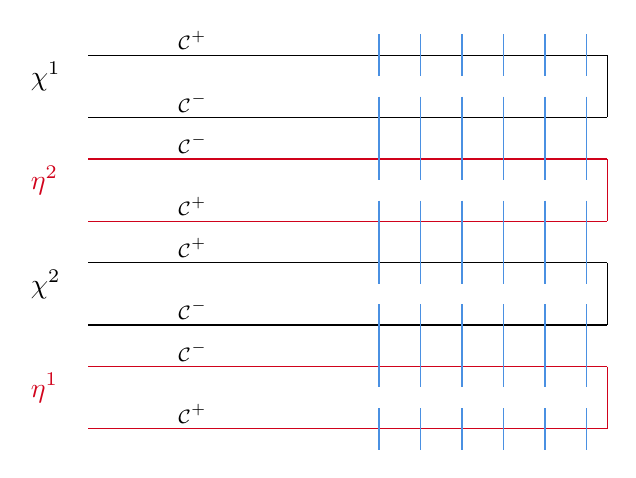
\begin{tikzpicture}[x=0.75pt,y=0.75pt,yscale=-1,xscale=1]

\draw    (90,30) -- (340,30) ;

\draw    (340,30) -- (340,60) ;

\draw    (90,60) -- (340,60) ;

\draw [color={rgb, 255:red, 208; green, 2; blue, 27 }  ,draw opacity=1 ]   (90,80) -- (340,80) ;

\draw [color={rgb, 255:red, 208; green, 2; blue, 27 }  ,draw opacity=1 ]   (340,80) -- (340,110) ;

\draw [color={rgb, 255:red, 208; green, 2; blue, 27 }  ,draw opacity=1 ]   (90,110) -- (340,110) ;

\draw    (90,130) -- (340,130) ;

\draw    (340,130) -- (340,160) ;

\draw    (90,160) -- (340,160) ;

\draw [color={rgb, 255:red, 208; green, 2; blue, 27 }  ,draw opacity=1 ]   (90,180) -- (340,180) ;

\draw [color={rgb, 255:red, 208; green, 2; blue, 27 }  ,draw opacity=1 ]   (340,180) -- (340,210) ;

\draw [color={rgb, 255:red, 208; green, 2; blue, 27 }  ,draw opacity=1 ]   (90,210) -- (340,210) ;

\draw [color={rgb, 255:red, 74; green, 144; blue, 226 }  ,draw opacity=1 ]   (230,50) -- (230,90) ;

\draw [color={rgb, 255:red, 74; green, 144; blue, 226 }  ,draw opacity=1 ]   (250,50) -- (250,90) ;

\draw [color={rgb, 255:red, 74; green, 144; blue, 226 }  ,draw opacity=1 ]   (270,50) -- (270,90) ;

\draw [color={rgb, 255:red, 74; green, 144; blue, 226 }  ,draw opacity=1 ]   (290,50) -- (290,90) ;

\draw [color={rgb, 255:red, 74; green, 144; blue, 226 }  ,draw opacity=1 ]   (310,50) -- (310,90) ;

\draw [color={rgb, 255:red, 74; green, 144; blue, 226 }  ,draw opacity=1 ]   (330,50) -- (330,90) ;

\draw [color={rgb, 255:red, 74; green, 144; blue, 226 }  ,draw opacity=1 ]   (230,100) -- (230,140) ;

\draw [color={rgb, 255:red, 74; green, 144; blue, 226 }  ,draw opacity=1 ]   (250,100) -- (250,140) ;

\draw [color={rgb, 255:red, 74; green, 144; blue, 226 }  ,draw opacity=1 ]   (270,100) -- (270,140) ;

\draw [color={rgb, 255:red, 74; green, 144; blue, 226 }  ,draw opacity=1 ]   (290,100) -- (290,140) ;

\draw [color={rgb, 255:red, 74; green, 144; blue, 226 }  ,draw opacity=1 ]   (310,100) -- (310,140) ;

\draw [color={rgb, 255:red, 74; green, 144; blue, 226 }  ,draw opacity=1 ]   (330,100) -- (330,140) ;

\draw [color={rgb, 255:red, 74; green, 144; blue, 226 }  ,draw opacity=1 ]   (230,150) -- (230,190) ;

\draw [color={rgb, 255:red, 74; green, 144; blue, 226 }  ,draw opacity=1 ]   (250,150) -- (250,190) ;

\draw [color={rgb, 255:red, 74; green, 144; blue, 226 }  ,draw opacity=1 ]   (270,150) -- (270,190) ;

\draw [color={rgb, 255:red, 74; green, 144; blue, 226 }  ,draw opacity=1 ]   (290,150) -- (290,190) ;

\draw [color={rgb, 255:red, 74; green, 144; blue, 226 }  ,draw opacity=1 ]   (310,150) -- (310,190) ;

\draw [color={rgb, 255:red, 74; green, 144; blue, 226 }  ,draw opacity=1 ]   (330,150) -- (330,190) ;

\draw [color={rgb, 255:red, 74; green, 144; blue, 226 }  ,draw opacity=1 ]   (230,200) -- (230,220) ;

\draw [color={rgb, 255:red, 74; green, 144; blue, 226 }  ,draw opacity=1 ]   (250,200) -- (250,220) ;

\draw [color={rgb, 255:red, 74; green, 144; blue, 226 }  ,draw opacity=1 ]   (270,200) -- (270,220) ;

\draw [color={rgb, 255:red, 74; green, 144; blue, 226 }  ,draw opacity=1 ]   (290,200) -- (290,220) ;

\draw [color={rgb, 255:red, 74; green, 144; blue, 226 }  ,draw opacity=1 ]   (310,200) -- (310,220) ;

\draw [color={rgb, 255:red, 74; green, 144; blue, 226 }  ,draw opacity=1 ]   (330,200) -- (330,220) ;

\draw [color={rgb, 255:red, 74; green, 144; blue, 226 }  ,draw opacity=1 ]   (230,20) -- (230,40) ;

\draw [color={rgb, 255:red, 74; green, 144; blue, 226 }  ,draw opacity=1 ]   (250,20) -- (250,40) ;

\draw [color={rgb, 255:red, 74; green, 144; blue, 226 }  ,draw opacity=1 ]   (270,20) -- (270,40) ;

\draw [color={rgb, 255:red, 74; green, 144; blue, 226 }  ,draw opacity=1 ]   (290,20) -- (290,40) ;

\draw [color={rgb, 255:red, 74; green, 144; blue, 226 }  ,draw opacity=1 ]   (310,20) -- (310,40) ;

\draw [color={rgb, 255:red, 74; green, 144; blue, 226 }  ,draw opacity=1 ]   (330,20) -- (330,40) ;

\draw (61,32) node [anchor=north west][inner sep=0.75pt]   [align=left] {$\displaystyle \chi^{1}$};

\draw (61,82) node [anchor=north west][inner sep=0.75pt]   [align=left] {$\displaystyle \textcolor[rgb]{0.82,0.01,0.11}{\eta^{2}}$};

\draw (61,132) node [anchor=north west][inner sep=0.75pt]   [align=left] {$\displaystyle \chi^{2}$};

\draw (61,182) node [anchor=north west][inner sep=0.75pt]   [align=left] {$\displaystyle \textcolor[rgb]{0.82,0.01,0.11}{\eta^{1}}$};

\draw (132,17) node [anchor=north west][inner sep=0.75pt]  [font=\scriptsize] [align=left] {$\displaystyle \mathcal{C}^{+}$};

\draw (132,47) node [anchor=north west][inner sep=0.75pt]  [font=\scriptsize] [align=left] {$\displaystyle \mathcal{C}^{-}$};

\draw (132,67) node [anchor=north west][inner sep=0.75pt]  [font=\scriptsize] [align=left] {$\displaystyle \mathcal{C}^{-}$};

\draw (132,97) node [anchor=north west][inner sep=0.75pt]  [font=\scriptsize] [align=left] {$\displaystyle \mathcal{C}^{+}$};

\draw (132,117) node [anchor=north west][inner sep=0.75pt]  [font=\scriptsize] [align=left] {$\displaystyle \mathcal{C}^{+}$};

\draw (132,147) node [anchor=north west][inner sep=0.75pt]  [font=\scriptsize] [align=left] {$\displaystyle \mathcal{C}^{-}$};

\draw (132,167) node [anchor=north west][inner sep=0.75pt]  [font=\scriptsize] [align=left] {$\displaystyle \mathcal{C}^{-}$};

\draw (132,197) node [anchor=north west][inner sep=0.75pt]  [font=\scriptsize] [align=left] {$\displaystyle \mathcal{C}^{+}$};

\end{tikzpicture}
    \caption{\textbf{From the \(\eta\)-twisted to the \(\chi\)-twisted
representation.}
The reduced-state contraction
\(\operatorname{Tr}_{\eta}(\sigma_{\eta,j}\rho_\eta)\) cyclically glues the
\(\eta\) indices between replicas, while the \(\chi\) indices close within
each replica. Regrouping the same wave-function coefficients as in
Eq.~\eqref{eq:S5-transition-identity} gives the identical contraction
\(\operatorname{Tr}_{\chi}
(\tau_{\chi,j}^{\dagger}\tau_{\chi,j})\), in which the \(\eta\) indices close
within each transition strip and the signed replica twist is carried by
\(\chi\). After the branch-dependent rotation in
Eq.~\eqref{eq:S5-branch-rotation}, this equivalence is represented by the
replica-diagonal pairings
\((\chi^{1},\eta^{1})\) and \((\chi^{2},\eta^{2})\) on
\(\mathcal C^{+}\), and the crossed pairings
\((\chi^{1},\eta^{2})\) and \((\chi^{2},\eta^{1})\) on
\(\mathcal C^{-}\). Red and black curves denote the \(\eta\) and \(\chi\)
contours, respectively, while the blue links indicate their mixed-interaction
pairing. Here \(R,L\) copy indices are suppressed.}
\label{fig:S5-eta-chi-twist}
\end{figure}

The two-replica bilocals in this frame are
\begin{equation}
\begin{aligned}
  (G^\eta_{ab})_{\alpha\beta}(z_1,z_2)
  &=
  -\frac{i}{N_\eta}
  \sum_{j=1}^{N_\eta}
  \eta^\alpha_{a,j}(z_1)
  \eta^\beta_{b,j}(z_2),
  \\
  (\widetilde G^\chi_{ab})_{\alpha\beta}(z_1,z_2)
  &=
  -\frac{i}{N_\chi}
  \sum_{k=1}^{N_\chi}
  \widetilde\chi^\alpha_{a,k}(z_1)
  \widetilde\chi^\beta_{b,k}(z_2).
\end{aligned}
\label{eq:S5-two-replica-bilocals}
\end{equation}
The physical \(\chi\) bilocal in the twisted frame is therefore
\begin{equation}
  G^{\chi,\mathrm{tw}}_{ab}(z_1,z_2)
  =
  \mathsf U^\dagger(z_1)
  \widetilde G^\chi_{ab}(z_1,z_2)
  \mathsf U(z_2).
\label{eq:S5-twisted-bath-bilocal}
\end{equation}
We rotate the bath self-energy in the same way,
\begin{equation}
  \Sigma^{\chi,\mathrm{tw}}_{ab}(z_1,z_2)
  =
  \mathsf U^\dagger(z_1)
  \widetilde\Sigma^\chi_{ab}(z_1,z_2)
  \mathsf U(z_2).
\label{eq:S5-twisted-bath-self-energy}
\end{equation}
Since \(\mathsf U\) is a real orthogonal signed-permutation matrix, the
componentwise bilocal pairing is invariant:
\begin{equation}
\begin{aligned}
  \sum_{\alpha,\beta}
  (\Sigma^{\chi,\mathrm{tw}}_{ab})_{\alpha\beta}
  (G^{\chi,\mathrm{tw}}_{ab})_{\alpha\beta}
  =
  \sum_{\alpha,\beta}
  (\widetilde\Sigma^\chi_{ab})_{\alpha\beta}
  (\widetilde G^\chi_{ab})_{\alpha\beta}.
\end{aligned}
\label{eq:S5-SigmaG-invariance}
\end{equation}

The kinetic and local left-right bilinear terms are also invariant under
Eq.~\eqref{eq:S5-untwisted-bath-field}. The pure \(\chi\) interaction is
invariant because left and right multiplication by \(\mathsf U\) only
permutes matrix entries and changes some signs, while \(p\) is even:
\begin{equation}
\begin{aligned}
  \sum_{\alpha,\beta}
  \left[
  2\left(
  \mathsf U^\dagger(z_1)
  \widetilde G^\chi_{ab}(z_1,z_2)
  \mathsf U(z_2)
  \right)_{\alpha\beta}
  \right]^p
  =
  \sum_{\alpha,\beta}
  \left[
  2(\widetilde G^\chi_{ab})_{\alpha\beta}(z_1,z_2)
  \right]^p .
\end{aligned}
\label{eq:S5-pure-bath-invariance}
\end{equation}
The rotation cannot be removed from the mixed interaction because the
\(\eta\) bilocal remains in the original replica frame. The
post-evaporation mixed combination is therefore
\begin{equation}
  s(G^\eta_{ab})_{\alpha\beta}
  +
  (1-s)
  (G^{\chi,\mathrm{tw}}_{ab})_{\alpha\beta}.
\label{eq:S5-mixed-bilocal}
\end{equation}

\paragraph*{Two-replica effective action and probe limit.}

The two-replica bare inverse propagator is the replica-diagonal lift of
Eq.~\eqref{eq:S-bare-inverse-propagator},
\begin{equation}
  (G_{0,2}^{-1})_{\alpha\beta;ab}(z_1,z_2)
  =
  \delta_{\alpha\beta}\,
  i\delta_{ab}\partial_{z_1}
  \delta_{\mathcal C}(z_1,z_2).
\label{eq:S5-bare-two-replica-propagator}
\end{equation}
Using the normalization of the one-replica action
\eqref{eq:S-effective-action}, the finite-\(s\), finite-\(p\) action in the
\(\chi\)-twisted representation is
\begin{equation}
\begin{aligned}
  \mathcal S_{\mathrm{2rep}}
  &=
  -s\frac{i}{2}
  \operatorname{Tr}\log
  \left[
  -i\left(G_{0,2}^{-1}-\Sigma^\eta\right)
  \right]
  -(1-s)\frac{i}{2}
  \operatorname{Tr}\log
  \left[
  -i\left(G_{0,2}^{-1}-\widetilde\Sigma^\chi\right)
  \right]
  \\
  &\quad
  +
  \frac{i}{2}
  \int_{\mathcal C}
  \mathrm dz_1\,\mathrm dz_2
  \sum_{a,b}
  \sum_{\alpha,\beta=1}^{2}
  \Big[
  s(\Sigma^\eta_{ab})_{\alpha\beta}
  (G^\eta_{ab})_{\alpha\beta}
  +
  (1-s)(\widetilde\Sigma^\chi_{ab})_{\alpha\beta}
  (\widetilde G^\chi_{ab})_{\alpha\beta}
  \Big]
  \\
  &\quad
  -
  \frac{i\mathcal J^2}{4p^2}
  \int_{\mathcal C}
  \mathrm dz_1\,\mathrm dz_2
  \sum_{a,b}
  \sum_{\alpha,\beta=1}^{2}
  (-1)^{1+p\delta_{ab}/2}
  \Bigg[
  l_\eta(z_1)l_\eta(z_2)
  \left[
  2(G^\eta_{ab})_{\alpha\beta}
  \right]^p
  \\
  &\hspace{3.2cm}
  +
  l_\chi(z_1)l_\chi(z_2)
  \left[
  2(\widetilde G^\chi_{ab})_{\alpha\beta}
  \right]^p
  \\
  &\hspace{3.2cm}
  +
  l_c(z_1)l_c(z_2)
  \Bigg\{
  \left[
  2\left(
  s(G^\eta_{ab})_{\alpha\beta}
  +
  (1-s)
  (G^{\chi,\mathrm{tw}}_{ab})_{\alpha\beta}
  \right)
  \right]^p
  \\
  &\hspace{5.5cm}
  -
  s^p
  \left[
  2(G^\eta_{ab})_{\alpha\beta}
  \right]^p
  -
  (1-s)^p
  \left[
  2(\widetilde G^\chi_{ab})_{\alpha\beta}
  \right]^p
  \Bigg\}
  \Bigg]
  \\
  &\quad
  +
  \frac{1}{2p}
  \int_{\mathcal C}
  \mathrm dz_1\,\mathrm dz_2\,
  \delta_{\mathcal C}(z_1,z_2)
  \sum_{\alpha=1}^{2}
  \Bigg[
  s\mu_\eta(z_1)
  \left(
  (G^\eta_{LR})_{\alpha\alpha}
  -
  (G^\eta_{RL})_{\alpha\alpha}
  \right)
  \\
  &\hspace{5.5cm}
  +
  (1-s)\mu_\chi(z_1)
  \left(
  (\widetilde G^\chi_{LR})_{\alpha\alpha}
  -
  (\widetilde G^\chi_{RL})_{\alpha\alpha}
  \right)
  \Bigg].
\end{aligned}
\label{eq:S5-two-replica-action}
\end{equation}
All bilocals in Eq.~\eqref{eq:S5-two-replica-action} are evaluated at
\((z_1,z_2)\) unless their arguments are shown explicitly. The trace in the
first line includes the contour, the \(R,L\) indices, and the replica
indices. The profiles \(l_\eta,l_\chi,l_c\) and
\(\mu_\eta,\mu_\chi\) are precisely those defined in
Eqs.~\eqref{eq:S-l-protocol} and \eqref{eq:S-bilinear-protocol}; no additional
bilinear-profile functions are introduced here.

For the two-replica calculation below, we work in the large-\(N\)
probe, or large-bath, limit
\begin{equation}
  N_\eta,N_\chi\longrightarrow\infty,
  \qquad
  s\longrightarrow0,
  \qquad
  b=d=1,
  \qquad
  p\ \text{fixed},\qquad p/2\ \text{even}.
\label{eq:S5-finite-p-probe-limit}
\end{equation}
At fixed \(p\), \(sp\to0\) follows from \(s\to0\), and the \(\chi\) saddle
has no backreaction from the \(\eta\) sector. Throughout the remainder of
this section, the two-replica equations are studied at finite \(p\).
An analytic treatment of the two-replica problem in the additional
large-\(p\) limit is left for future work.

In the untwisted frame the bath saddle is replica diagonal:
\begin{equation}
  (\widetilde G^\chi_{ab})_{\alpha\beta}(z_1,z_2)
  =
  \delta_{\alpha\beta}\,
  G^\chi_{ab}(z_1,z_2),
\label{eq:S5-replica-diagonal-bath}
\end{equation}
where \(G^\chi_{ab}\) is the ordinary one-replica bath solution of
Eqs.~\eqref{eq:S-contour-dyson} and \eqref{eq:S-self-energy}. Transforming
back to the physical twisted frame gives
\begin{equation}
  (G^{\chi,\mathrm{tw}}_{ab})_{\alpha\beta}(z_1,z_2)
  =
  G^\chi_{ab}(z_1,z_2)\,
  \Pi_{\alpha\beta}(z_1,z_2),
  \qquad
  \Pi(z_1,z_2)
  \equiv
  \mathsf U^\dagger(z_1)\mathsf U(z_2).
\label{eq:S5-twist-kernel}
\end{equation}
Explicitly,
\begin{equation}
  \Pi(z_1,z_2)
  =
  \begin{cases}
    \mathbf 1,
    &z_1,z_2\in\mathcal C_{\rm u}
    \ \text{or}\
    z_1,z_2\in\mathcal C_{\rm l},
    \\[4pt]
    \mathsf S,
    &z_1\in\mathcal C_{\rm u},
    \quad
    z_2\in\mathcal C_{\rm l},
    \\[4pt]
    \mathsf S^\dagger=-\mathsf S,
    &z_1\in\mathcal C_{\rm l},
    \quad
    z_2\in\mathcal C_{\rm u}.
  \end{cases}
\label{eq:S5-twist-kernel-cases}
\end{equation}
Every entry of \(\Pi\) is \(0\) or \(\pm1\). Since \(p-1\) is odd,
the elementwise power appearing in the self-energy satisfies
\begin{equation}
  \left[
  2G^\chi_{ab}(z_1,z_2)
  \Pi(z_1,z_2)
  \right]^{\circ(p-1)}
  =
  \left[
  2G^\chi_{ab}(z_1,z_2)
  \right]^{p-1}
  \Pi(z_1,z_2),
\label{eq:S5-twist-power}
\end{equation}
where the superscript \(\circ(p-1)\) denotes an elementwise power in replica
space.

For the sharp protocol, let \(\mathcal C_<\) denote the Euclidean preparation
segments together with the real-time portions before \(t_{\rm ev}\), and let
\(\mathcal C_>\) denote the real-time portions after \(t_{\rm ev}\). Varying
Eq.~\eqref{eq:S5-two-replica-action} and taking the limit
\eqref{eq:S5-finite-p-probe-limit} gives
\begin{equation}
\begin{aligned}
  (\Sigma^\eta_{ab})_{\alpha\beta}(z_1,z_2)
  &=
  (-1)^{1+p\delta_{ab}/2}
  \frac{\mathcal J^2}{p}
  \begin{cases}
    a^2
    \left[
    2(G^\eta_{ab})_{\alpha\beta}(z_1,z_2)
    \right]^{p-1},
    &z_1,z_2\in\mathcal C_<,
    \\[6pt]
    \left[
    2G^\chi_{ab}(z_1,z_2)
    \right]^{p-1}
    \Pi_{\alpha\beta}(z_1,z_2),
    &z_1,z_2\in\mathcal C_>,
    \\[6pt]
    0,
    &z_1\in\mathcal C_<,\ z_2\in\mathcal C_>
    \ \text{or vice versa}
  \end{cases}
  \\
  &\quad
  -
  i\epsilon_{ab}\,
  \delta_{\alpha\beta}\,
  \frac{\mu_\eta(z_1)}{p}
  \delta_{\mathcal C}(z_1,z_2),
\end{aligned}
\label{eq:S5-probe-self-energy}
\end{equation}
where \(\epsilon_{ab}\) is defined in Eq.~\eqref{eq:S-epsilon}. The
pre-evaporation replica problem retains the nonlinear \(\eta\) self-energy,
whereas after evaporation the \(\eta\) probe is driven by the known scalar
bath solution multiplied by the signed replica kernel \(\Pi\). There is no
interaction self-energy when the two arguments lie on opposite sides of the
evaporation surface. The probe calculation therefore requires no new
nonlinear bath saddle.

\paragraph*{Numerical two-replica equations.}

The scalar bath correlator \(G^\chi\) is first obtained from the ordinary
one-replica equations \eqref{eq:S-contour-dyson} and
\eqref{eq:S-self-energy}. The resulting bath solution is then held fixed
while solving the two-replica \(\eta\) equation.

Discretize the contour by points \(z_i\), ordered so that
\(i>j\) means \(z_i>_{\mathcal C}z_j\). Each fold contains a Euclidean
preparation segment of target length \(\beta/4\) and a real-time segment
ending at \(t_f\). The implementation uses real-time spacing \(\Delta t\)
and chooses the integer node counts as follows:

\begin{equation}
  N_\beta
  =
  \operatorname{round}\!\left(\frac{\beta}{4\Delta t}\right),
  \qquad
  N_t
  =
  \operatorname{round}\!\left(\frac{t_f}{\Delta t}\right),
  \qquad
  N_{\rm fold}
  =
  N_\beta+N_t,
  \qquad
  N_{\mathcal C}
  =
  2N_{\rm fold}.
\label{eq:S5-grid-sizes}
\end{equation}
The plotted final times are grid aligned, so \(N_t\Delta t=t_f\).
The Euclidean spacing is chosen separately as
\(\Delta\tau=\beta/(4N_\beta)\), so that each preparation segment
has length \(N_\beta\Delta\tau=\beta/4\) and
\(\beta_{\rm grid}=4N_\beta\Delta\tau=\beta\), up to floating-point precision.
For Fig.~\ref{main-fig:finite_p}, \(\beta=5.7355465869\) and
\(\Delta t=0.5\) give \(N_\beta=3\) and
\(\Delta\tau\simeq0.4779622156\). The contour measure is represented
by the diagonal weight matrix
\begin{equation}
  W^{ab}_{ij}
  =
  \delta_{ab}\delta_{ij}w_i,
  \qquad
  w_i
  =
  \begin{cases}
    -i\Delta\tau,
    &0\leq i<N_\beta,
    \\[2pt]
    +\Delta t,
    &N_\beta\leq i<N_{\rm fold},
    \\[2pt]
    -\Delta t,
    &N_{\rm fold}\leq i<N_{\rm fold}+N_t,
    \\[2pt]
    -i\Delta\tau,
    &N_{\rm fold}+N_t\leq i<2N_{\rm fold}.
  \end{cases}
\label{eq:S5-contour-weights}
\end{equation}

Using the composite index
\[
  \mathcal A=(\alpha,a,i),
  \qquad
  \alpha=1,2,
  \quad
  a\in\{R,L\},
  \quad
  i=0,\ldots,N_{\mathcal C}-1,
\]
the replica-diagonal free propagator and weight matrix are
\begin{equation}
\begin{aligned}
  (\mathbf G_{0,2})_{\alpha a i,\beta b j}
  &=
  \delta_{\alpha\beta}
  (\mathbf G_0)_{a i,b j},
  \\
  (\mathbf W_2)_{\alpha a i,\beta b j}
  &=
  \delta_{\alpha\beta}\delta_{ab}\delta_{ij}w_i .
\end{aligned}
\label{eq:S5-discrete-replica-lift}
\end{equation}
At the discrete level the signed twist is
\begin{equation}
  \Pi_{ij}
  =
  \mathsf U^\dagger(z_i)\mathsf U(z_j).
\label{eq:S5-discrete-twist}
\end{equation}

Let \(T_i\) be the real time associated with \(z_i\), with Euclidean
preparation points assigned to the pre-evaporation region. Define the masks
\begin{equation}
\begin{aligned}
  M_{\rm I}(i,j)
  &=
  \mathbf 1_{T_i\leq t_{\rm ev}}
  \mathbf 1_{T_j\leq t_{\rm ev}},
  \\
  M_{\rm III}(i,j)
  &=
  \mathbf 1_{T_i>t_{\rm ev}}
  \mathbf 1_{T_j>t_{\rm ev}},
  \\
  M_{\rm II}(i,j)
  &=
  1-M_{\rm I}(i,j)-M_{\rm III}(i,j).
\end{aligned}
\label{eq:S5-region-masks}
\end{equation}
Here \(\mathbf 1\) is an indicator function. A grid point exactly at
\(t_{\rm ev}\) belongs to the pre-evaporation region, so the masks form a
partition also on the quench slice.
The pre-evaporation self-energy is nonlinear in the unknown two-replica
correlator:
\begin{equation}
  \left(
  \Sigma^{\eta,\rm I}_{ab}
  \right)_{\alpha\beta;ij}
  =
  M_{\rm I}(i,j)
  (-1)^{1+p\delta_{ab}/2}
  \frac{a^2\mathcal J^2}{p}
  \left[
  2(G^\eta_{ab})_{\alpha\beta;ij}
  \right]^{p-1}.
\label{eq:S5-discrete-sigma-I}
\end{equation}
The post-evaporation self-energy is fixed by the bath:
\begin{equation}
  \left(
  \Sigma^{\eta,\rm III}_{ab}
  \right)_{\alpha\beta;ij}
  =
  M_{\rm III}(i,j)
  (-1)^{1+p\delta_{ab}/2}
  \frac{\mathcal J^2}{p}
  \left[
  2G^\chi_{ab;ij}
  \right]^{p-1}
  (\Pi_{ij})_{\alpha\beta}.
\label{eq:S5-discrete-sigma-III}
\end{equation}
There is no interaction contribution in region II. A local \(\eta\)
bilinear, if retained, is represented by
\begin{equation}
  (\mathbf V_\eta)_{\alpha a i,\beta b j}
  =
  -i\epsilon_{ab}\,
  \delta_{\alpha\beta}\delta_{ij}
  \frac{\mu_\eta(z_i)}{p}.
\label{eq:S5-discrete-bilinear}
\end{equation}
For the protocol used in the numerical results,
\(\mu_\eta=0\), so \(\mathbf V_\eta=0\).

The discrete two-replica Dyson equation is
\begin{equation}
\begin{aligned}
  \mathbf G_\eta
  &=
  \mathbf G_{0,2}
  +
  \mathbf G_{0,2}
  \Big[
  \mathbf W_2\mathbf V_\eta
  +
  \mathbf W_2
  \left(
  \boldsymbol\Sigma^{\eta,\rm I}[\mathbf G_\eta]
  +
  \boldsymbol\Sigma^{\eta,\rm III}_{\chi}
  \right)
  \mathbf W_2
  \Big]
  \mathbf G_\eta .
\end{aligned}
\label{eq:S5-discrete-Dyson}
\end{equation}
The local vertex carries one contour weight, whereas a nonlocal bilocal
self-energy carries one weight for each contour argument.

Because the post-evaporation bath source is fixed, define
\begin{equation}
  \mathbf A_\chi
  =
  \mathbf 1
  -
  \mathbf G_{0,2}
  \left[
  \mathbf W_2\mathbf V_\eta
  +
  \mathbf W_2
  \boldsymbol\Sigma^{\eta,\rm III}_{\chi}
  \mathbf W_2
  \right].
\label{eq:S5-fixed-bath-operator}
\end{equation}
The remaining nonlinear residual is
\begin{equation}
\begin{aligned}
  R_\eta(\mathbf G_\eta)
  &=
  \mathbf A_\chi\mathbf G_\eta
  -
  \mathbf G_{0,2}
  -
  \mathbf G_{0,2}
  \mathbf W_2
  \boldsymbol\Sigma^{\eta,\rm I}[\mathbf G_\eta]
  \mathbf W_2
  \mathbf G_\eta .
\end{aligned}
\label{eq:S5-replica-residual}
\end{equation}
We solve \(R_\eta=0\) using a damped Newton--Krylov method. The
Jacobian-vector product is
\begin{equation}
\begin{aligned}
  J_\eta[\mathbf G_\eta]\mathbf X
  &=
  \mathbf A_\chi\mathbf X
  -
  \mathbf G_{0,2}\mathbf W_2
  \delta\boldsymbol\Sigma^{\eta,\rm I}[\mathbf X]
  \mathbf W_2\mathbf G_\eta
  -
  \mathbf G_{0,2}\mathbf W_2
  \boldsymbol\Sigma^{\eta,\rm I}[\mathbf G_\eta]
  \mathbf W_2\mathbf X ,
\end{aligned}
\label{eq:S5-replica-JVP}
\end{equation}
where
\begin{equation}
\begin{aligned}
  \left(
  \delta\Sigma^{\eta,\rm I}_{ab}[\mathbf X]
  \right)_{\alpha\beta;ij}
  &=
  M_{\rm I}(i,j)
  (-1)^{1+p\delta_{ab}/2}
  \frac{a^2\mathcal J^2}{p}
  (p-1)\,2
  \left[
  2(G^\eta_{ab})_{\alpha\beta;ij}
  \right]^{p-2}
  (X_{ab})_{\alpha\beta;ij}.
\end{aligned}
\label{eq:S5-replica-delta-sigma}
\end{equation}
At each Newton step, we use the generalized minimal residual method (GMRES) to solve the linearized equation
\(J_\eta[\mathbf G_\eta]\delta\mathbf G_\eta
=-R_\eta(\mathbf G_\eta)\). The solver requires only the Jacobian-vector
product in Eq.~\eqref{eq:S5-replica-JVP}, so the full Jacobian is never
constructed. Starting from the linearized residual \(\mathbf r\), GMRES
builds the Krylov subspace
\(\operatorname{span}\{\mathbf r,J_\eta\mathbf r,\ldots,
J_\eta^{m-1}\mathbf r\}\) and chooses the correction that minimizes the
residual norm within this subspace. In practice, \(\mathbf A_\chi^{-1}\) is used as a preconditioner: it
approximately removes the stiff linear contribution from the fixed bath,
improving the conditioning of the linear system and accelerating GMRES
without changing the desired solution.

If \(i_-(t_b)\) and \(i_+(t_b)\) are the lower- and upper-branch indices
corresponding to \(t_b\), the normalized overlap is read off as
\begin{equation}
  F_2(t_b;t_f)
  =
  2i\,
  (\mathbf G_\eta)_{
  (1,R,i_-(t_b)),
  (2,R,i_+(t_b))
  }.
\label{eq:S5-discrete-F2-readout}
\end{equation}

\paragraph*{R\'enyi-2 mutual information.}

For compactness, define the branch-resolved contractions
\begin{equation}
  C_{\alpha\beta}^{\lambda_1\lambda_2}(t_b;t_f)
  \equiv
  2i\,
  G^{(2),\eta;\chi\text{-tw}}_{RR;\alpha\beta}
  (t_{b,\lambda_1},t_{b,\lambda_2};t_f),
  \qquad
  \lambda_1,\lambda_2\in\{+,-\}.
\label{eq:S5-branch-contractions}
\end{equation}
Thus
\begin{equation}
  F_2(t_b;t_f)
  =
  C_{12}^{-+}(t_b;t_f).
\label{eq:S5-F2-C}
\end{equation}

The second contraction required below is the fixed-flavor perturbed purity,
averaged over the flavor index:
\begin{equation}
  F_4(t_b;t_f)
  =
  \frac{1}{N_\eta}
  \sum_{j=1}^{N_\eta}
  \frac{
  \operatorname{Tr}_{\eta}
  \left[
  \sigma_{\eta,j}(t_b;t_f)^2
  \right]
  }{
  \mathcal P_\eta(t_f)
  } .
\label{eq:S5-F4-density}
\end{equation}
At leading order in large \(N_\eta\), the corresponding four-point
function factorizes into two-replica two-point functions. Keeping the
fermionic Wick signs gives
\begin{equation}
\begin{aligned}
  F_4(t_b;t_f)
  &=
  C_{11}^{-+}(t_b;t_f)
  C_{22}^{-+}(t_b;t_f)
  -
  C_{12}^{-+}(t_b;t_f)
  C_{21}^{-+}(t_b;t_f)
  -
  C_{12}^{--}(t_b;t_f)
  C_{12}^{++}(t_b;t_f).
\end{aligned}
\label{eq:S5-F4-green}
\end{equation}
The last term pairs the two lower-branch insertions with each other and the
two upper-branch insertions with each other. Thus no independent four-point
saddle is required.

The corresponding \(\chi\)-side cross contraction is
\begin{equation}
\begin{aligned}
  K_2(t_b;t_f)
  &=
  \frac{1}{N_\eta}
  \sum_{j=1}^{N_\eta}
  \frac{
  \operatorname{Tr}_{\chi}
  \left[
  \sigma_{\chi,j}(t_b;t_f)
   \rho_\chi(t_f)
  \right]
  }{
  \mathcal P_\chi(t_f)
  }
  \\
  &=
  C_{11}^{-+}(t_b;t_f)
  =
  2i\,
  G^{(2),\eta;\chi\text{-tw},>}_{RR;11}
  (t_b,t_b;t_f).
\end{aligned}
\label{eq:S5-K2}
\end{equation}

To retain the coherence of the infalling excitation, introduce an auxiliary
two-dimensional reference system \(P\) and purify the choice of whether or
not the simple fermion was inserted:
\begin{equation}
  \lvert\Omega_j(t_f)\rangle_{P\eta\chi}
  =
  \frac{1}{\sqrt{2}}
  \left[
  \lvert0\rangle_P
  \lvert\Phi(t_f)\rangle_{\eta\chi}
  +
  \lvert1\rangle_P
  \lvert\Phi_{b,j}(t_f)\rangle_{\eta\chi}
  \right].
\label{eq:S5-reference-state}
\end{equation}
Since \(\eta^R_j(t_b)\) is fermion odd, the states
\(\lvert\Phi(t_f)\rangle\) and
\(\lvert\Phi_{b,j}(t_f)\rangle\) have opposite fermion parity and are
therefore orthogonal. It follows that the reference system is maximally
mixed:
\begin{equation}
  \rho_P
  =
  \frac{1}{2}
  \left(
  \lvert0\rangle\langle0\rvert
  +
  \lvert1\rangle\langle1\rvert
  \right),
  \qquad
  S_P^{(2)}
  =
  -\log\operatorname{Tr}\rho_P^2
  =
  \log2 .
\label{eq:S5-reference-entropy}
\end{equation}

The R\'enyi-2 mutual-information diagnostic between \(P\) and \(\eta\) is
\begin{equation}
  I^{(2)}(P:\eta)
  =
  S_P^{(2)}
  +
  S_\eta^{(2)}
  -
  S_{P\eta}^{(2)}.
\label{eq:S5-MI-definition}
\end{equation}
The full \(P\eta\chi\) state is pure, so
\(S_{P\eta}^{(2)}=S_\chi^{(2)}\). Therefore
\begin{equation}
\begin{aligned}
  e^{-I^{(2)}(P:\eta)}
  &=
  \frac{
  \operatorname{Tr}_{\eta}
  \left[
  \left(
  \rho_\eta+\sigma_{\eta,j}
  \right)^2
  \right]
  }{
  2\operatorname{Tr}_{\chi}
  \left[
  \left(
  \rho_\chi+\sigma_{\chi,j}
  \right)^2
  \right]
  }
  \\
  &=
  \frac{1}{2}
  \frac{
  1+2F_2+F_4
  }{
  1+2K_2+F_4
  }.
\end{aligned}
\label{eq:S5-MI-ratio}
\end{equation}
The first line is precisely the density-matrix expression quoted in
Eq.~\eqref{main-eq:renyi2_MI}. The second line uses flavor symmetry at the
leading disorder-averaged large-\(N\) saddle, where the fixed-flavor
contractions equal \(F_2,F_4,K_2\); it is not an identity between averages
of ratios in an arbitrary finite-\(N\) realization. In the ideal limit in which \(P\) and the retained
\(\eta\) information are maximally entangled, this diagnostic equals
\(2\log2\).

\paragraph*{Projection onto the reconstructed bulk mode.}

Equations~\eqref{eq:S5-F2-green}, \eqref{eq:S5-F4-green}, and
\eqref{eq:S5-K2} were written first for a simple boundary insertion. The
main-text result instead uses the reconstructed infalling mode
\(\psi_{R,f}(u,t_{\rm max})\). According to
Eq.~\eqref{main-eq:HKLL_kernel}, this operator is a linear combination of
boundary operators over the reconstruction interval.

Let \(\mathbf K_f(u,t_{\rm max})\) denote the corresponding discretized
reconstruction row, including the boundary-copy components used in the
reconstruction. For an insertion on the ket or upper branch and on the bra
or lower branch, respectively, use
\begin{equation}
  \mathbf K_f^{(+)}
  =
  \mathbf K_f,
  \qquad
  \mathbf K_f^{(-)}
  =
  \mathbf K_f^*.
\label{eq:S5-kernel-branch-rule}
\end{equation}
If
\(\mathbf C_{\alpha\beta}^{\lambda_1\lambda_2}\)
denotes the branch-resolved two-replica correlator matrix assembled from the
\(RR,RL,LR,LL\) boundary blocks, define its bulk projection by
\begin{equation}
  C_{\alpha\beta}^{\lambda_1\lambda_2}
  [\mathbf K_f]
  =
  \mathbf K_f^{(\lambda_1)}
  \mathbf C_{\alpha\beta}^{\lambda_1\lambda_2}
  \left(
  \mathbf K_f^{(\lambda_2)}
  \right)^T .
\label{eq:S5-kernel-projection}
\end{equation}
A boundary insertion at \(t_b\) is recovered by taking
\(\mathbf K_f\) to be the corresponding delta-function row. For the
reconstructed bulk mode, the quantities entering the mutual information are
\begin{equation}
\begin{aligned}
  F_2[\mathbf K_f]
  &=
  C_{12}^{-+}[\mathbf K_f],
  \\
  K_2[\mathbf K_f]
  &=
  C_{11}^{-+}[\mathbf K_f],
  \\
  F_4[\mathbf K_f]
  &=
  C_{11}^{-+}[\mathbf K_f]
  C_{22}^{-+}[\mathbf K_f]
  -
  C_{12}^{-+}[\mathbf K_f]
  C_{21}^{-+}[\mathbf K_f]
  -
  C_{12}^{--}[\mathbf K_f]
  C_{12}^{++}[\mathbf K_f].
\end{aligned}
\label{eq:S5-bulk-contractions}
\end{equation}
Substitution of these kernel-projected contractions into
Eq.~\eqref{eq:S5-MI-ratio} gives the bulk-mode R\'enyi-2 mutual information
shown in Fig.~\ref{main-fig:finite_p}.

\paragraph*{On-shell action and second R\'enyi entropy.}

The unperturbed two-replica saddles also determine the second R\'enyi entropy
of the full \(\eta\) sector. Let the statistical on-shell action be
\begin{equation}
  \mathcal I
  =
  -i\,
  \mathcal S_{\mathrm{2rep,on\mbox{-}shell}},
\label{eq:S5-statistical-action}
\end{equation}
where the contour action includes both Euclidean preparation segments and
both real-time branches. The contour weights in
Eq.~\eqref{eq:S5-contour-weights} already include all branch orientations.

The purity is the ratio of the \(\chi\)-twisted partition function to the
disconnected two-replica partition function:
\begin{equation}
  \operatorname{Tr}\rho_\eta(t_f)^2
  =
  \frac{
  Z_{\chi\text{-tw}}(t_f)
  }{
  Z_{\rm disc}(t_f)
  }
  \sim
  \exp
  \left[
  -(N_\eta+N_\chi)
  \left(
  \mathcal I_{\chi\text{-tw}}
  -
  \mathcal I_{\rm disc}
  \right)
  \right].
\label{eq:S5-purity-action-ratio}
\end{equation}
In the probe limit the statistical action has the expansion
\begin{equation}
  \mathcal I
  =
  \mathcal I_\chi
  +
  s\,i_\eta
  +
  O(s^2),
  \qquad
  s
  =
  \frac{N_\eta}{N_\eta+N_\chi}.
\label{eq:S5-probe-action-expansion}
\end{equation}
The bath saddle is common to the twisted and disconnected solutions at this
order, so its contribution cancels. Define
\begin{equation}
  \Delta i_\eta(t_f)
  =
  i_{\eta,\chi\text{-tw}}(t_f)
  -
  i_{\eta,\rm disc}(t_f).
\label{eq:S5-delta-action}
\end{equation}
The entropy normalization is then
\begin{equation}
  \frac{
  S_\eta^{(2)}(t_f)
  }{
  N_\eta
  }
  =
  \operatorname{Re}\Delta i_\eta(t_f),
  \qquad
  \frac{
  S_\eta^{(2)}(t_f)
  }{
  N_\eta+N_\chi
  }
  =
  s\,
  \operatorname{Re}\Delta i_\eta(t_f).
\label{eq:S5-entropy-normalization}
\end{equation}
Here
\(S_\eta^{(2)}(t_f)
=-\log\operatorname{Tr}\rho_\eta(t_f)^2\).
The imaginary part of \(\Delta i_\eta\) is a numerical convergence
diagnostic and should vanish for a converged physical saddle.

The doubled \(\eta\) system contains \(2N_\eta\) Majorana fermions and has
Hilbert-space dimension \(2^{N_\eta}\). Consequently,
\begin{equation}
  0
  \leq
  \frac{S_\eta^{(2)}(t_f)}{N_\eta}
  =
  \operatorname{Re}\Delta i_\eta(t_f)
  \leq
  \log2.
\label{eq:S5-entropy-bound}
\end{equation}

For the \(\chi\)-twisted saddle, the post-evaporation source is the one in
Eq.~\eqref{eq:S5-discrete-sigma-III}. The disconnected saddle uses the same
scalar bath correlator but no replica mixing:
\begin{equation}
  \left(
  \Sigma^{\eta,\rm III}_{\rm disc,ab}
  \right)_{\alpha\beta;ij}
  =
  M_{\rm III}(i,j)
  (-1)^{1+p\delta_{ab}/2}
  \frac{\mathcal J^2}{p}
  \left[
  2G^\chi_{ab;ij}
  \right]^{p-1}
  \delta_{\alpha\beta}.
\label{eq:S5-disconnected-source}
\end{equation}
For the convention used in the plots, \(p/2\) is even, so
\((-1)^{1+p\delta_{ab}/2}=-1\) in every \(R,L\) block. We also use
\(\mathbf V_\eta=0\).

The free determinant is identical for the twisted and disconnected saddles.
Writing
\[
  G_{0,2}^{-1}-\Sigma^\eta
  =
  G_{0,2}^{-1}
  \left(
  \mathbf 1-G_{0,2}\Sigma^\eta
  \right)
\]
makes this cancellation explicit. The UV-subtracted discrete
log-determinant contribution is
\begin{equation}
\begin{aligned}
  i_{\eta,\log}
  &=
  -\frac{1}{2}
  \log\det
  \left[
  \mathbf 1
  -
  \mathbf G_{0,2}
  \mathbf W_2
  \left(
  \boldsymbol\Sigma^{\eta,\rm I}
  +
  \boldsymbol\Sigma^{\eta,\rm III}
  \right)
  \mathbf W_2
  \right].
\end{aligned}
\label{eq:S5-relative-logdet}
\end{equation}
Both contour arguments of a nonlocal self-energy carry a quadrature weight.

At leading order in the probe expansion, the explicit region-III
\(\Sigma G\) contribution cancels the region-III mixed potential. The
post-evaporation self-energy nevertheless remains in the determinant and in
the saddle equation. The surviving pre-evaporation interaction contribution
is
\begin{equation}
\begin{aligned}
  i_{\eta,\rm I}
  &=
  \frac{a^2\mathcal J^2}{4p^2}
  \sum_{\alpha,\beta=1}^{2}
  \sum_{a,b=R,L}
  \sum_{i,j}
  w_iw_j\,
  M_{\rm I}(i,j)
  (-1)^{1+p\delta_{ab}/2}
  \left[
  2(G^\eta_{ab})_{\alpha\beta;ij}
  \right]^p .
\end{aligned}
\label{eq:S5-early-interaction-action}
\end{equation}
The corresponding constraint contribution is
\begin{equation}
\begin{aligned}
  i_{\Sigma_{\rm I}G}
  &=
  \frac{1}{2}
  \sum_{\alpha,\beta=1}^{2}
  \sum_{a,b=R,L}
  \sum_{i,j}
  w_iw_j\,
  \left(
  \Sigma^{\eta,\rm I}_{ab}
  \right)_{\alpha\beta;ij}
  \left(
  G^\eta_{ab}
  \right)_{\alpha\beta;ij}.
\end{aligned}
\label{eq:S5-SigmaG-action}
\end{equation}
This is an elementwise bilocal contraction; it should not be replaced by an
ordinary matrix trace, which reverses one of the matrix indices.

The \(\eta\)-normalized probe action evaluated on either saddle is therefore
\begin{equation}
  i_\eta
  =
  i_{\eta,\log}
  +
  i_{\Sigma_{\rm I}G}
  -
  i_{\eta,\rm I}.
\label{eq:S5-probe-action}
\end{equation}
For each \(t_f\), the required action difference is
\begin{equation}
\begin{aligned}
  \Delta i_\eta(t_f)
  &=
  i_\eta
  \left[
  G^\eta_{\chi\text{-tw}};
  \Sigma^{\eta,\rm III}_{\chi\text{-tw}}
  \right]
  -
  i_\eta
  \left[
  G^\eta_{\rm disc};
  \Sigma^{\eta,\rm III}_{\rm disc}
  \right].
\end{aligned}
\label{eq:S5-final-action-difference}
\end{equation}

Finally, at fixed contour extent and fixed discretization,
\(\Sigma^\eta=O(p^{-1})\) gives the formal large-\(p\) expansion of the
relative determinant (the series converges when the spectral radius of
\(\mathbf A\) is less than one):
\begin{equation}
  -\frac{1}{2}\log\det(\mathbf 1-\mathbf A)
  =
  \frac{1}{2}\operatorname{Tr}\mathbf A
  +
  \frac{1}{4}\operatorname{Tr}\mathbf A^2
  +
  \cdots,
  \qquad
  \mathbf A
  =
  \mathbf G_{0,2}
  \mathbf W_2
  \boldsymbol\Sigma^\eta
  \mathbf W_2 .
\label{eq:S5-logdet-expansion}
\end{equation}
Accordingly,
\begin{equation}
  \Delta i_\eta(t_f)
  =
  \frac{c_1(t_f)}{p}
  +
  \frac{c_2(t_f)}{p^2}
  +
  O(p^{-3}),
\label{eq:S5-large-p-action-scaling}
\end{equation}
unless an additional symmetry removes the leading coefficient. At fixed final time, this gives
the large-\(p\) scaling
\(S_\eta^{(2)}=O(N_\eta/p)\) quoted in the main text. The numerical
consistency checks are
\begin{equation}
  \operatorname{Re}\Delta i_\eta\geq0,
  \qquad
  \operatorname{Im}\Delta i_\eta\simeq0,
  \qquad
  \Delta i_\eta(t_f\leq t_{\rm ev})=0,
  \qquad
  \operatorname{Re}\Delta i_\eta\leq\log2.
\label{eq:S5-action-checks}
\end{equation}

\section*{S6. Large-\(p\) conventions, Lensky-Qi parametrization, and the left-right bound}
\paragraph*{Reflection symmetry and the large-\(p\) ansatz.}

We first collect the symmetry, normalization, and branch conventions used in
Secs.~S2-S5. For either species
\(\psi\in\{\eta,\chi\}\), and for \(p/2\) even, the doubled Hamiltonian is invariant under
\begin{equation}
\mathbf R[\psi_R]=-\psi_L,
\qquad
\mathbf R[\psi_L]=\psi_R .
\label{eq:S6-reflection}
\end{equation}
The bilinear \(\psi_L\psi_R\) is invariant under the same transformation.

For real times, define
\begin{equation}
G^{\psi,>}_{ab}(t_1,t_2)
=
-i\left\langle
\psi_a(t_1)\psi_b(t_2)
\right\rangle,
\qquad
a,b\in\{R,L\}.
\label{eq:S6-Wightman-definition}
\end{equation}
Hermiticity and reflection symmetry imply
\begin{equation}
\begin{aligned}
\left[
G^{\psi,>}_{ab}(t_1,t_2)
\right]^*
&=
-G^{\psi,>}_{ba}(t_2,t_1),
\\
G^{\psi,>}_{LL}(t_1,t_2)
&=
G^{\psi,>}_{RR}(t_1,t_2),
\qquad
G^{\psi,>}_{LR}(t_1,t_2)
=
-G^{\psi,>}_{RL}(t_1,t_2).
\end{aligned}
\label{eq:S6-Wightman-symmetries}
\end{equation}
Consequently,
\begin{equation}
\begin{aligned}
G^{\psi,>}_{RR}(t_1,t_2)
&=
-\left[
G^{\psi,>}_{RR}(t_2,t_1)
\right]^*,
\\
G^{\psi,>}_{RL}(t_1,t_2)
&=
\left[
G^{\psi,>}_{RL}(t_2,t_1)
\right]^* .
\end{aligned}
\label{eq:S6-independent-components}
\end{equation}
For complex contour times, Hermiticity becomes
\begin{equation}
\left[
G^{\psi,>}_{ab}(z_1,z_2)
\right]^*
=
-G^{\psi,>}_{ba}(z_2^*,z_1^*) .
\label{eq:S6-complex-Wightman-conjugation}
\end{equation}

The normalization and form of the large-\(p\) ansatz can be motivated from the free
bilinear problem
\begin{equation}
\label{eq:app-free-bilinear-hamiltonian}
  H_{\mathrm{bil}}=i\mu \psi_L\psi_R .
\end{equation}
Here \(\mu\) is the physical single-pair gap; in the large-\(p\) scaling of the model it is replaced by \(\mu_\psi/p\).
With
\begin{equation}
\label{eq:app-free-c}
  c=\frac{\psi_L+i\psi_R}{\sqrt{2}},
  \qquad
  c^\dagger=\frac{\psi_L-i\psi_R}{\sqrt{2}},
\end{equation}
one has
\begin{equation}
\label{eq:app-free-spectrum}
  H_{\mathrm{bil}}
  =
  \mu\left(c^\dagger c-\frac{1}{2}\right).
\end{equation}
In a thermal state \(\rho=e^{-\beta H_{\mathrm{bil}}}/Z_\beta\),
\begin{equation}
\label{eq:app-free-GRR}
  G^{>}_{RR}(t,0)
  =
  -\frac{i}{2}
  \frac{
  \cosh\left[\frac{\mu}{2}(\beta-2it)\right]
  }{
  \cosh\left(\frac{\beta\mu}{2}\right)
  }
  \xrightarrow{\beta\mu\to\infty}
  -\frac{i}{2}e^{-i\mu t},
\end{equation}
and
\begin{equation}
\label{eq:app-free-GRL}
  G^{>}_{RL}(t,0)
  =
  -\frac{1}{2}
  \frac{
  \sinh\left[\frac{\mu}{2}(\beta-2it)\right]
  }{
  \cosh\left(\frac{\beta\mu}{2}\right)
  }
  \xrightarrow{\beta\mu\to\infty}
  -\frac{1}{2}e^{-i\mu t}.
\end{equation}
This motivates the large-\(p\) parametrization
\begin{equation}
\begin{aligned}
G^{\psi,>}_{RR}(t_1,t_2)
&=
-\frac{i}{2}
e^{g^\psi_R(t_1,t_2)/p}
=
G^{\psi,>}_{LL}(t_1,t_2),
\\
G^{\psi,>}_{RL}(t_1,t_2)
&=
-\frac{1}{2}
e^{g^\psi_L(t_1,t_2)/p}
=
-G^{\psi,>}_{LR}(t_1,t_2).
\end{aligned}
\label{eq:S6-large-p-components}
\end{equation}
Thus the subscript \(R\) on \(g^\psi_R\) denotes the diagonal
\(RR/LL\) channel, whereas \(L\) on \(g^\psi_L\) denotes the off-diagonal
\(RL/LR\) channel.

We choose the continuous logarithmic branch for which
\(g^\psi_{R,L}=O(1)\) as \(p\to\infty\). Equations
\eqref{eq:S6-independent-components} and
\eqref{eq:S6-large-p-components} then give
\begin{equation}
g^\psi_X(t_1,t_2)
=
\left[
g^\psi_X(t_2,t_1)
\right]^*,
\qquad
X=R,L .
\label{eq:S6-real-time-g-conjugation}
\end{equation}
On the complex contour,
\begin{equation}
\left[
g^\psi_X(z_1,z_2)
\right]^*
=
g^\psi_X(z_2^*,z_1^*),
\qquad
X=R,L .
\label{eq:S6-complex-time-g-conjugation}
\end{equation}
In particular,
\begin{equation}
g^\psi_R(t,t)=0,
\qquad
g^\psi_L(t,t)\in\mathbb R .
\label{eq:S6-equal-time-g}
\end{equation}
These relations fix the conjugation and branch conventions used in the
matching formulas of Sec.~S3.

\paragraph*{Lensky-Qi parametrization.}

Consider a real-time region in which the correlators satisfy the homogeneous
Liouville equations with effective interaction scale
\(\mathcal J_{\mathrm{eff}}\),
\begin{equation}
\partial_{t_1}\partial_{t_2}g_X(t_1,t_2)
=
2\sigma_X\mathcal J_{\mathrm{eff}}^{\,2}
e^{g_X(t_1,t_2)},
\qquad
\sigma_R=1,
\qquad
\sigma_L=-1 .
\label{eq:S6-LQ-Liouville}
\end{equation}
For the bath,
\(\mathcal J_{\mathrm{eff}}=\mathcal J\), whereas for the
pre-evaporation \(\eta\) solution,
\(\mathcal J_{\mathrm{eff}}=a\mathcal J\).

Following Lensky and Qi \cite{lensky2021rescuing}, the physical solution
selected by the thermal gluing conditions
\eqref{eq:S-large-p-gluing} and the equal-time data
\eqref{eq:S-equal-time-R} and \eqref{eq:S-equal-time-L} may be described by
a single complex function \(y(t)\):
\begin{equation}
\begin{aligned}
e^{g_R(t_1,t_2)}
&=
-
\frac{
y'(t_1)y'(t_2)^*
}{
\sin^2\left(
\mathcal J_{\mathrm{eff}}
\left[y(t_1)-y(t_2)^*\right]
\right)
},
\\
e^{g_L(t_1,t_2)}
&=
\frac{
y'(t_1)y'(t_2)^*
}{
\cos^2\left(
\mathcal J_{\mathrm{eff}}
\left[y(t_1)-y(t_2)^*\right]
\right)
}.
\end{aligned}
\label{eq:S6-LQ-parametrization}
\end{equation}
The variable denoted by \(y\) here is denoted by \(\psi\) in
Ref.~\cite{lensky2021rescuing}; we use \(y\) to avoid confusion with the
species label \(\psi\in\{\eta,\chi\}\). Its dimensions are
\begin{equation}
[y]=[t]=[\mathcal J_{\mathrm{eff}}]^{-1}.
\label{eq:S6-y-dimension}
\end{equation}

We choose the physical lower-half-plane branch
\begin{equation}
\operatorname{Im}y(t)<0 .
\label{eq:S6-physical-branch}
\end{equation}
The equal-time normalization \(g_R(t,t)=0\) then requires
\begin{equation}
|y'(t)|
=
\sinh\left(
2\mathcal J_{\mathrm{eff}}
|\operatorname{Im}y(t)|
\right).
\label{eq:S6-y-normalization}
\end{equation}

It is useful to introduce real variables \(\phi(t)\) and \(p(t)\) by
\begin{equation}
y'(t)
=
|y'(t)|e^{ip(t)}
=
\frac{
e^{ip(t)}
}{
\sqrt{e^{2\phi(t)}-1}
}.
\label{eq:S6-y-phase-parametrization}
\end{equation}
Here \(p(t)\) is the Lensky--Qi canonical phase conjugate to \(\phi(t)\); it
should not be confused with the interaction order \(p\). The equal-time
left-right correlator is
\begin{equation}
g_L(t,t)=-2\phi(t).
\label{eq:S6-gL-phi}
\end{equation}

For a real bilinear coupling \(\mu_{\mathrm{eff}}(t)\), the variables
\((\phi,p)\) evolve according to the classical Hamiltonian
\begin{equation}
\mathcal H_Q(\phi,p;t)
=
-2\mathcal J_{\mathrm{eff}}
\sqrt{1-e^{-2\phi}}\cos p
+
\mu_{\mathrm{eff}}(t)\phi,
\qquad
\{\phi,p\}_{\mathrm{P.B.}}=1 .
\label{eq:S6-LQ-Hamiltonian}
\end{equation}
The corresponding Hamilton equations are
\begin{equation}
\begin{aligned}
\dot\phi
&=
2\mathcal J_{\mathrm{eff}}
\sqrt{1-e^{-2\phi}}\sin p,
\\
\dot p
&=
-\mu_{\mathrm{eff}}(t)
+
2\mathcal J_{\mathrm{eff}}
\frac{
e^{-2\phi}
}{
\sqrt{1-e^{-2\phi}}
}
\cos p .
\end{aligned}
\label{eq:S6-LQ-Hamilton-equations}
\end{equation}

\paragraph*{Lensky-Qi trajectories used in Secs.~S3 and S4.}

For the pre-evaporation \(\eta\) segment,
\(\mathcal J_{\mathrm{eff}}=a\mathcal J\) and
\(\mu_{\mathrm{eff}}=0\). In terms of the thermal angle \(\vartheta\) defined
in Eq.~\eqref{eq:S3-thermal-angle}, the corresponding trajectory is
\begin{equation}
\begin{aligned}
\phi_\eta(t)
&=
\log\left[
\frac{
\cosh\left(
2a\mathcal Jt\sin\vartheta
\right)
}{
\sin\vartheta
}
\right],
\\
p_\eta(t)
&=
\tan^{-1}\left[
\tan\vartheta\,
\tanh\left(
2a\mathcal Jt\sin\vartheta
\right)
\right],
\\
y_\eta(t)
&=
\frac{1}{a\mathcal J}
\tan^{-1}
\tanh\left(
a\mathcal Jt\sin\vartheta
-\frac{i\vartheta}{2}
\right).
\end{aligned}
\label{eq:S6-eta-trajectory}
\end{equation}
The inverse functions and logarithms in this expression are taken on their
continuous branches. Substitution into
Eq.~\eqref{eq:S6-LQ-parametrization} reproduces the pre-evaporation
correlators in Eq.~\eqref{eq:S3-eta-pre}.

For the stationary traversable-wormhole bath,
\(\mathcal J_{\mathrm{eff}}=\mathcal J\) and
\(\mu_{\mathrm{eff}}=\mu_0\). It is the fixed point
\begin{equation}
\phi_\chi(t)=\phi_G,
\qquad
p_\chi(t)=0,
\label{eq:S6-chi-fixed-point}
\end{equation}
where \(\phi_G\) and \(V_G\) are defined in
Eq.~\eqref{eq:S3-bath-parameters}. A convenient representative of the
corresponding \(y\)-trajectory is
\begin{equation}
y_\chi(t)
=
V_G(t-t_\star)
-
\frac{i}{2\mathcal J}
\tanh^{-1}(r_G),
\qquad
V_G
=
\frac{r_G}{\sqrt{1-r_G^2}},
\label{eq:S6-chi-trajectory}
\end{equation}
where \(t_\star\) is an arbitrary time origin. Substitution into
Eq.~\eqref{eq:S6-LQ-parametrization} reproduces the stationary bath
correlators in Eq.~\eqref{eq:S3-bath-solution}.

\paragraph*{Disk-coordinate proof of the post-evaporation bound.}

We now prove Eq.~\eqref{eq:S3-post-L-ratio-bound} under the assumptions of
Eq.~\eqref{eq:S3-LQ-bound-assumptions}, with \(h_\chi\) defined in
Eq.~\eqref{eq:S3-post-L-ratio}. In this paragraph
\(g_{R,L}=g^\chi_{R,L}\), and therefore
\(\mathcal J_{\mathrm{eff}}=\mathcal J\).

Introduce the disk coordinate
\begin{equation}
w(t)
=
e^{-2i\mathcal J y(t)}.
\label{eq:S6-disk-coordinate}
\end{equation}
Because \(\operatorname{Im}y(t)<0\),
\begin{equation}
|w(t)|
=
e^{2\mathcal J\operatorname{Im}y(t)}
<1 .
\label{eq:S6-disk-interior}
\end{equation}
Equation~\eqref{eq:S6-y-normalization} becomes
\begin{equation}
|y'(t)|
=
\frac{
1-|w(t)|^2
}{
2|w(t)|
}.
\label{eq:S6-yprime-disk}
\end{equation}

For \(w_a=w(t_a)\) and \(w_b=w(t_b)\),
\begin{equation}
\begin{aligned}
\left|
\sin\left(
\mathcal J[y(t_a)-y(t_b)^*]
\right)
\right|^2
&=
\frac{
|1-w_aw_b^*|^2
}{
4|w_a||w_b|
},
\\
\left|
\cos\left(
\mathcal J[y(t_a)-y(t_b)^*]
\right)
\right|^2
&=
\frac{
|1+w_aw_b^*|^2
}{
4|w_a||w_b|
}.
\end{aligned}
\label{eq:S6-disk-trigonometric-identities}
\end{equation}
Define the disk invariant
\begin{equation}
\mathcal P(u,v)
\equiv
\frac{
(1-|u|^2)(1-|v|^2)
}{
|1-uv^*|^2
}.
\label{eq:S6-disk-kernel}
\end{equation}
It is invariant under simultaneous automorphisms of the unit disk.
Equations~\eqref{eq:S6-LQ-parametrization},
\eqref{eq:S6-yprime-disk}, and
\eqref{eq:S6-disk-trigonometric-identities} give
\begin{equation}
\left|e^{g^\chi_R(t_a,t_b)}\right|
=
\mathcal P(w_a,w_b),
\qquad
\left|e^{g^\chi_L(t_a,t_b)}\right|
=
\mathcal P(w_a,-w_b).
\label{eq:S6-correlators-disk}
\end{equation}

Let
\begin{equation}
w_i=w(t_i),
\qquad
w_{\rm ev}=w(t_{\rm ev}).
\end{equation}
Substitution into Eq.~\eqref{eq:S3-post-L-ratio} gives
\begin{equation}
h_\chi
=\mathcal P(w_1,-w_2)
\mathcal P(w_{\rm ev},-w_{\rm ev})
\frac{\mathcal P(w_1,w_{\rm ev})
\mathcal P(w_2,w_{\rm ev})
}{
\mathcal P(w_1,-w_{\rm ev})
\mathcal P(w_2,-w_{\rm ev})
}.
\label{eq:S6-h-disk}
\end{equation}
Here and below the arguments
\((t_1,t_2;t_{\rm ev})\) of \(h_\chi\) are suppressed.

Apply the disk automorphism
\begin{equation}
z(w)
=
\frac{
w-w_{\rm ev}
}{
1-w_{\rm ev}^*w
}.
\label{eq:S6-disk-automorphism}
\end{equation}
It obeys
\begin{equation}
z(w_{\rm ev})=0,
\qquad
z(-w_{\rm ev})=-v,
\qquad
z(-w)
=
-\frac{
z(w)+v
}{
1+v^*z(w)
}, \qquad {\text{where~}}
v
=
\frac{
2w_{\rm ev}
}{
1+|w_{\rm ev}|^2
}.
\label{eq:S6-disk-images}
\end{equation}
Because \(|w_{\rm ev}|<1\), one has \(|v|<1\).

Writing
\begin{equation}
z_j=z(w_j),
\qquad
z'_j=z(-w_j),
\end{equation}
the invariance of \(\mathcal P\) reduces Eq.~\eqref{eq:S6-h-disk} to
\begin{equation}
h_\chi
=
\frac{
\mathcal P(z_1,0)\mathcal P(z_2,0)
}{
\mathcal P(z'_1,0)\mathcal P(z'_2,0)
}
\mathcal P(z_1,z'_2)\mathcal P(v,0).
\label{eq:S6-h-transformed}
\end{equation}
Using Eq.~\eqref{eq:S6-disk-images} explicitly gives
\begin{equation}
h_\chi
=
\frac{
(1-|z_1|^2)(1-|z_2|^2)
|1+z_1v^*|^2
|1+z_2v^*|^2
}{
|1+z_1v^*+z_2^*v+z_1z_2^*|^2
}.
\label{eq:S6-h-z}
\end{equation}

Remove the phase of \(v\) by writing
\begin{equation}
v=\rho e^{i\alpha_0},
\qquad
\rho=|v|<1,
\qquad
\tau_j=e^{-i\alpha_0}z_j ,
\label{eq:S6-phase-rotation}
\end{equation}
with an arbitrary choice of \(\alpha_0\) if \(v=0\). Then
\begin{equation}
h_\chi
=
\frac{
(1-|\tau_1|^2)(1-|\tau_2|^2)
|1+\rho\tau_1|^2
|1+\rho\tau_2|^2
}{
\left|
1+\rho\tau_1+\rho\tau_2^*
+\tau_1\tau_2^*
\right|^2
},
\qquad
|\tau_1|,|\tau_2|<1 .
\label{eq:S6-h-canonical-disk-form}
\end{equation}
Notice that \(h_\chi\) is already a nonnegative modulus; the ratio in
Eq.~\eqref{eq:S6-h-canonical-disk-form} is \(h_\chi\), not \(h_\chi^2\).

To bound this expression, define
\begin{equation}
\kappa
=
\frac{
\rho+\tau_1
}{
1+\rho\tau_1
}.
\label{eq:S6-CS-kappa}
\end{equation}
Since \(\rho\) is real,
\begin{equation}
1-|\kappa|^2
=
\frac{
(1-\rho^2)(1-|\tau_1|^2)
}{
|1+\rho\tau_1|^2
}
>0,
\label{eq:S6-CS-kappa-disk}
\end{equation}
so \(\kappa\) lies in the open unit disk. Moreover,
\begin{equation}
1+\rho\tau_1+\rho\tau_2^*
+\tau_1\tau_2^*
=
(1+\rho\tau_1)
(1+\kappa\tau_2^*).
\label{eq:S6-CS-factorization}
\end{equation}
Consequently,
\begin{equation}
h_\chi
=
(1-|\tau_2|^2)
\left|F(\tau_2)\right|^2,
\label{eq:S6-CS-h-F}
\end{equation}
where
\begin{equation}
F(\lambda)
=
\sqrt{1-|\tau_1|^2}\,
\frac{
1+\rho\lambda
}{
1+\kappa^*\lambda
}.
\label{eq:S6-CS-function}
\end{equation}
Because \(|\kappa|<1\), \(F\) is holomorphic on the unit disk. Its Taylor
series is
\begin{equation}
F(\lambda)
=
\sqrt{1-|\tau_1|^2}
\left[
1+
(\rho-\kappa^*)
\sum_{n=1}^{\infty}
(-\kappa^*)^{n-1}\lambda^n
\right].
\label{eq:S6-CS-series}
\end{equation}
Writing
\begin{equation}
F(\lambda)=\sum_{n=0}^{\infty}d_n\lambda^n,
\end{equation}
the coefficients are
\begin{equation}
d_0
=
\sqrt{1-|\tau_1|^2},
\qquad
d_n
=
\sqrt{1-|\tau_1|^2}
(\rho-\kappa^*)
(-\kappa^*)^{n-1},
\quad n\geq1 .
\label{eq:S6-CS-coefficients}
\end{equation}

The associated Hardy norm is therefore finite and equals
\begin{equation}
\begin{aligned}
\|F\|_{H^2}^2
&\equiv
\sum_{n=0}^{\infty}|d_n|^2
\\
&=
(1-|\tau_1|^2)
\left[
1+
\frac{
|\rho-\kappa^*|^2
}{
1-|\kappa|^2
}
\right].
\end{aligned}
\label{eq:S6-CS-Hardy-norm}
\end{equation}
Since \(\rho\) is real,
\begin{equation}
\rho-\kappa
=
-\frac{
(1-\rho^2)\tau_1
}{
1+\rho\tau_1
},
\qquad
|\rho-\kappa^*|
=
|\rho-\kappa|.
\label{eq:S6-CS-rho-minus-kappa}
\end{equation}
Combining Eqs.~\eqref{eq:S6-CS-kappa-disk} and
\eqref{eq:S6-CS-rho-minus-kappa} gives
\begin{equation}
\|F\|_{H^2}^2
=
1-\rho^2|\tau_1|^2
\leq1 .
\label{eq:S6-CS-Hardy-norm-final}
\end{equation}

Because \(F\in H^2\), Cauchy--Schwarz applied to its Taylor series gives
\begin{equation}
\begin{aligned}
|F(\tau_2)|^2
&=
\left|
\sum_{n=0}^{\infty}
d_n\tau_2^n
\right|^2
\\
&\leq
\left(
\sum_{n=0}^{\infty}|d_n|^2
\right)
\left(
\sum_{n=0}^{\infty}|\tau_2|^{2n}
\right)
\\
&=
\frac{
\|F\|_{H^2}^2
}{
1-|\tau_2|^2
}.
\end{aligned}
\label{eq:S6-CS-evaluation}
\end{equation}
Using Eq.~\eqref{eq:S6-CS-h-F}, we obtain
\begin{equation}
h_\chi
\leq
\|F\|_{H^2}^2
=
1-\rho^2|\tau_1|^2
\leq1 .
\label{eq:S6-CS-first-bound}
\end{equation}
The canonical expression
\eqref{eq:S6-h-canonical-disk-form} is invariant under complex conjugation
combined with exchange of the two insertion points. Applying the same
argument after this exchange gives
\begin{equation}
h_\chi
\leq
1-\rho^2|\tau_2|^2
\leq1 .
\label{eq:S6-CS-second-bound}
\end{equation}
Since \(h_\chi\) is nonnegative by definition,
\begin{equation}
0
\leq
h_\chi(t_1,t_2;t_{\rm ev})
\leq
1 .
\label{eq:S6-h-bound}
\end{equation}
This proves Eq.~\eqref{eq:S3-post-L-ratio-bound}. Together with
Eq.~\eqref{eq:S3-post-L-magnitude}, it establishes
Eq.~\eqref{eq:S3-post-L-bound}.

% BEGIN REFERENCES
\begin{thebibliography}{1}
\expandafter\ifx\csname url\endcsname\relax
  \def\url#1{\burl{#1}}\fi
\expandafter\ifx\csname urlprefix\endcsname\relax\def\urlprefix{URL }\fi
\providecommand{\bibinfo}[2]{#2}
\providecommand{\eprint}[2][]{\url{#2}}
\providecommand{\doi}[1]{\url{https://doi.org/#1}}

\bibitem{maldacena2018eternal}
\bibinfo{author}{Maldacena, J.} \& \bibinfo{author}{Qi, X.-L.}
\newblock \bibinfo{title}{{Eternal traversable wormhole}}.
\newblock \emph{\bibinfo{journal}{arXiv preprint arXiv:1804.00491}}
  (\bibinfo{year}{2018}).

\bibitem{lensky2021rescuing}
\bibinfo{author}{Lensky, Y.~D.} \& \bibinfo{author}{Qi, X.-L.}
\newblock \bibinfo{title}{{Rescuing a black hole in the large-q coupled SYK
  model}}.
\newblock \emph{\bibinfo{journal}{Journal of High Energy Physics}}
  \textbf{\bibinfo{volume}{2021}}, \bibinfo{pages}{116} (\bibinfo{year}{2021}).

\end{thebibliography}
% END REFERENCES
\end{document}
